\documentclass[journal]{IEEEtran}
\ifCLASSINFOpdf
  \usepackage[pdftex]{graphicx}  
\else
\fi

% correct bad hyphenation here
\hyphenation{op-tical net-works semi-conduc-tor}
\usepackage[colorlinks=true]{hyperref}
\usepackage{amssymb}
\usepackage{algorithm}
\usepackage{amsmath}
\let\proof\relax
\let\endproof\relax
\usepackage{amsthm}
\usepackage{graphicx}
\usepackage{subfigure}
\usepackage{tabularx}
\usepackage{booktabs}
\usepackage{url}
\usepackage{bbm}
\usepackage[noend]{algpseudocode}
\usepackage{array}
\usepackage{balance}
\usepackage{multirow}
\usepackage{multicol}
\usepackage{threeparttable}
%\usepackage{cite}
\usepackage{subfigure}
\allowdisplaybreaks
\newcommand\algotext[1]{\end{algorithmic}#1\begin{algorithmic}[1]}


\newcommand{\var}{{\rm var}}
\newcommand{\Tr}{^{\top}}
\newcommand{\vtrans}[2]{{#1}^{(#2)}}
\newcommand{\kron}{\otimes}
\newcommand{\schur}[2]{({#1} | {#2})}
\newcommand{\schurdet}[2]{\left| ({#1} | {#2}) \right|}
\newcommand{\had}{\circ}
\newcommand{\diag}{{\rm diag}}
\newcommand{\invdiag}{\diag^{-1}}
\newcommand{\rank}{{\rm rank}}
\newcommand{\expt}[1]{\langle #1 \rangle}
% careful: ``null'' is already a latex command
\newcommand{\nullsp}{{\rm null}}
\newcommand{\tr}{{\rm tr}}
\renewcommand{\vec}{{\rm vec}}
\newcommand{\vech}{{\rm vech}}
\renewcommand{\det}[1]{\left| #1 \right|}
\newcommand{\pdet}[1]{\left| #1 \right|_{+}}
\newcommand{\pinv}[1]{#1^{+}}
\newcommand{\erf}{{\rm erf}}
\newcommand{\hypergeom}[2]{{}_{#1}F_{#2}}
\newcommand{\mcal}[1]{\mathcal{#1}}
\newcommand{\Rcal}{{\mathcal{R}}}
\newcommand{\Acal}{{\mathcal{A}}}
\newcommand{\Ecal}{{\mathcal{E}}}
\newcommand{\Fcal}{{\mathcal{F}}}
\newcommand{\Ncal}{{\mathcal{N}}}
\newcommand{\Vcal}{{\mathcal{V}}}
% boldface characters
\renewcommand{\a}{{\bf a}}
\renewcommand{\b}{{\bf b}}
\renewcommand{\c}{{\bf c}}
\renewcommand{\d}{{\rm d}}  % for derivatives
\newcommand{\e}{{\bf e}}
\newcommand{\f}{{\bf f}}
\newcommand{\g}{{\bf g}}
\newcommand{\h}{{\bf h}}
\newcommand{\bi}{{\bf i}}
\newcommand{\bj}{{\bf j}}
\newcommand{\bK}{{\bf K}}
%\newcommand{\k}{{\bf k}}
% in Latex2e this must be renewcommand
\renewcommand{\k}{{\bf k}}
\newcommand{\m}{{\bf m}}
\newcommand{\mhat}{{\overline{m}}}
\newcommand{\tm}{{\tilde{m}}}
\newcommand{\n}{{\bf n}}
\renewcommand{\o}{{\bf o}}
\newcommand{\p}{{\bf p}}
\newcommand{\q}{{\bf q}}
\renewcommand{\r}{{\bf r}}
\newcommand{\s}{{\bf s}}
\renewcommand{\t}{{\bf t}}
\renewcommand{\u}{{\bf u}}
\renewcommand{\v}{{\bf v}}
\newcommand{\w}{{\bf w}}
\newcommand{\x}{{\bf x}}
\newcommand{\y}{{\bf y}}
\newcommand{\z}{{\bf z}}
\newcommand{\bl}{{\bf l}}
\newcommand{\A}{{\bf A}}
\newcommand{\B}{{\bf B}}
%\newcommand{\C}{{\bf C}}
\newcommand{\D}{{\bf D}}
\newcommand{\Dcal}{\mathcal{D}}
\newcommand{\E}{{\bf E}}
\newcommand{\F}{{\bf F}}
%\newcommand{\G}{{\bf G}}
\newcommand{\Gcal}{{\mathcal{G}}}
\renewcommand{\H}{{\bf H}}
\newcommand{\I}{{\bf I}}
\newcommand{\J}{{\bf J}}
\newcommand{\K}{{\bf K}}
\renewcommand{\L}{{\bf L}}
%\newcommand{\Lcal}{{\mathcal{L}}}
\newcommand{\M}{{\bf M}}
\newcommand{\Mcal}{{\mathcal{M}}}
\newcommand{\N}{{\bf N}}
\newcommand{\bupeta}{\boldsymbol{\upeta}}
\renewcommand{\O}{{\bf O}}
\renewcommand{\P}{{\bf P}}
\newcommand{\Q}{{\bf Q}}
\newcommand{\R}{{\bf R}}
\renewcommand{\S}{{\bf S}}
\newcommand{\Scal}{{\mathcal{S}}}
\newcommand{\T}{{\bf T}}
\newcommand{\Tcal}{{\mathcal{T}}}
%\newcommand{\U}{{\bf U}}
\newcommand{\Ucal}{{\mathcal{U}}}
\newcommand{\tU}{{\tilde{\U}}}
\newcommand{\tUcal}{{\tilde{\Ucal}}}
\newcommand{\V}{{\bf V}}
\newcommand{\W}{{\bf W}}

\newcommand{\Ocal}[1]{{\mathcal{O}\left(#1\right)}}
\newcommand{\Pcal}{{\mathcal{P}}}
\newcommand{\WScal}{{\mathcal{WS}}}
\newcommand{\Hcal}{{\mathcal{H}}}
\newcommand{\Wcal}{{\mathcal{W}}}
\newcommand{\X}{{\bf X}}
\newcommand{\Xcal}{{\mathcal{X}}}
\newcommand{\Y}{{\bf Y}}
\newcommand{\Ycal}{{\mathcal{Y}}}
\newcommand{\Z}{{\bf Z}}
\newcommand{\Zcal}{{\mathcal{Z}}}

\newcommand{\Lcal}{{\mathcal{L}}}

% this is for latex 2.09
% unfortunately, the result is slanted - use Latex2e instead
%\newcommand{\bfLambda}{\mbox{\boldmath$\Lambda$}}
% this is for Latex2e
\newcommand{\bfLambda}{\boldsymbol{\Lambda}}

% Yuan Qi's boldsymbol
\newcommand{\bsigma}{\boldsymbol{\sigma}}
\newcommand{\balpha}{\boldsymbol{\alpha}}
\newcommand{\bpsi}{\boldsymbol{\psi}}
\newcommand{\bphi}{\boldsymbol{\phi}}
\newcommand{\bbeta}{\boldsymbol{\beta}}
\newcommand{\bepsi}{\boldsymbol{\epsilon}}
\newcommand{\Beta}{\boldsymbol{\eta}}
\newcommand{\btau}{\boldsymbol{\tau}}
\newcommand{\bvarphi}{\boldsymbol{\varphi}}
\newcommand{\bzeta}{\boldsymbol{\zeta}}

\newcommand{\blambda}{\boldsymbol{\lambda}}
\newcommand{\bLambda}{\mathbf{\Lambda}}
\newcommand{\bdelta}{\boldsymbol{\delta}}
\newcommand{\bDelta}{\mathbf{\Delta}}
\newcommand{\btheta}{\boldsymbol{\theta}}
\newcommand{\bTheta}{\boldsymbol{\Theta}}
\newcommand{\bpi}{\boldsymbol{\pi}}
\newcommand{\bxi}{\boldsymbol{\xi}}
\newcommand{\bSigma}{\boldsymbol{\Sigma}}
\newcommand{\bPi}{\boldsymbol{\Pi}}
\newcommand{\bOmega}{\boldsymbol{\Omega}}
%\newcommand{\bLambda}{\boldsymbol{\Lambda}}

\newcommand{\bnu}{\boldsymbol{\nu}}

\newcommand{\hatu}{\hat{\bf u}}



\newcommand{\bgamma}{\boldsymbol{\gamma}}
\newcommand{\bGamma}{\boldsymbol{\Gamma}}
\newcommand{\bUpsilon}{\boldsymbol{\Upsilon}}



\newcommand{\bmu}{\boldsymbol{\mu}}
\newcommand{\1}{{\bf 1}}
\newcommand{\0}{{\bf 0}}


\newcommand{\proj}[1]{{\rm proj}\negmedspace\left[#1\right]}
\newcommand{\argmin}{\operatornamewithlimits{argmin}}
\newcommand{\argmax}{\operatornamewithlimits{argmax}}

\newcommand{\dif}{\mathrm{d}}
\newcommand{\lrincir}[1]{\left( #1 \right)}
\newcommand{\abs}[1]{\lvert#1\rvert}
\newcommand{\norm}[1]{\lVert#1\rVert}
\newcommand{\lrnorm}[1]{\left\lVert#1\right\rVert}
\newcommand{\lrangle}[1]{\left\langle#1 \right\rangle}

\newcommand{\ie}{{{i.e.,}}\xspace}
\newcommand{\eg}{{{\em e.g.,}}\xspace}
\newcommand{\EE}{\mathop{\mathbb{E}}}
\newcommand{\RR}{\mathbb{R}}
\newcommand{\sbr}[1]{\left[#1\right]}
\newcommand{\rbr}[1]{\left(#1\right)}
%\newcommand{\Lcal}[1]{\mathcal{L}^{#1}_{D_1,D_2}}


\newcommand{\refabove}[2]{\displaystyle_{#1}^{(#2)}}
\newcommand{\refabovecir}[2]{\displaystyle_{#1}^{#2}}

\newtheorem{Definition}{\bf{Definition}}
\newtheorem{Property}{\bf{Property}}
\newtheorem{Theorem}{\bf{Theorem}}
\newtheorem{Corollary}{\bf{Corollary}}
\newtheorem{Lemma}{\bf{Lemma}}
\newtheorem{Remark}{\bf{Remark}}
\newtheorem{Assumption}{\bf{Assumption}}
\begin{document}


\title{Communication Efficient Training of Federated Model Over Unbalanced Labels}


\author{Yawei Zhao, Qinghe Liu, Mingming Jiang, Kunlun He
\thanks{Yawei Zhao, Qinghe Liu, Mingming Jiang, and Kunlun He are with the Medical Big Data Research Center, Chinese PLA General Hospital, Beijing, 100039, China. E-mail: \texttt{csyawei.zhao@gmail.com},  \texttt{Liuqinghe9638@163.com}, \texttt{jiangmingming1994@163.com}, \texttt{kunlunhe@plagh.org}.
}
}



% make the title area
\maketitle

% As a general rule, do not put math, special symbols or citations
% in the abstract or keywords.
\begin{abstract}
xxx

\end{abstract}

% Note that keywords are not normally used for peerreview papers.
\begin{IEEEkeywords}
xxxx
\end{IEEEkeywords}


\IEEEpeerreviewmaketitle


\section{Introduction}
\label{sect_introduction}
xxx




\section{Formulation}

\subsection{Personalized Representation based on Similarity Network}

Personalized models are built based on the similarity network. The similarity network measures the similarity of data distribution under data/feature/model space.  
\begin{itemize}
\item \textbf{Data space.} In the case, local datasets of every node are used to construct a \textit{kernel} matrix. The similarity of data distribution is measured by xxxxx.
\item \textbf{Feature space.} In the case, local datasets of every node are used to construct a \textit{covariance} matrix. It represents the dependence structure among features. The similarity of data distribution is measured based on the distance between covariance matrices.
\item \textbf{Model space.} In the case, local model of every node is trained by using the local dataset. The similarity of data distribution is measured based on the distance between local models.
\end{itemize}

Based on similarity under those space, the similarity network $\Gcal = \{\Ncal, \Ecal\}$ is built by using the KNN method \cite{dd}. $\Ncal=\{1,2, ..., N\}$ represents the node set, consisting of $N$ nodes. $\Ecal=\{e_{i,j} : i\in\Ncal, j {~} \text{is the node $i$'s neighbour}\}$ represents the edge set, consisting of $M$ edges. 

\begin{figure}[!t]
\setlength{\abovecaptionskip}{0pt}
\setlength{\belowcaptionskip}{0pt}
\centering 
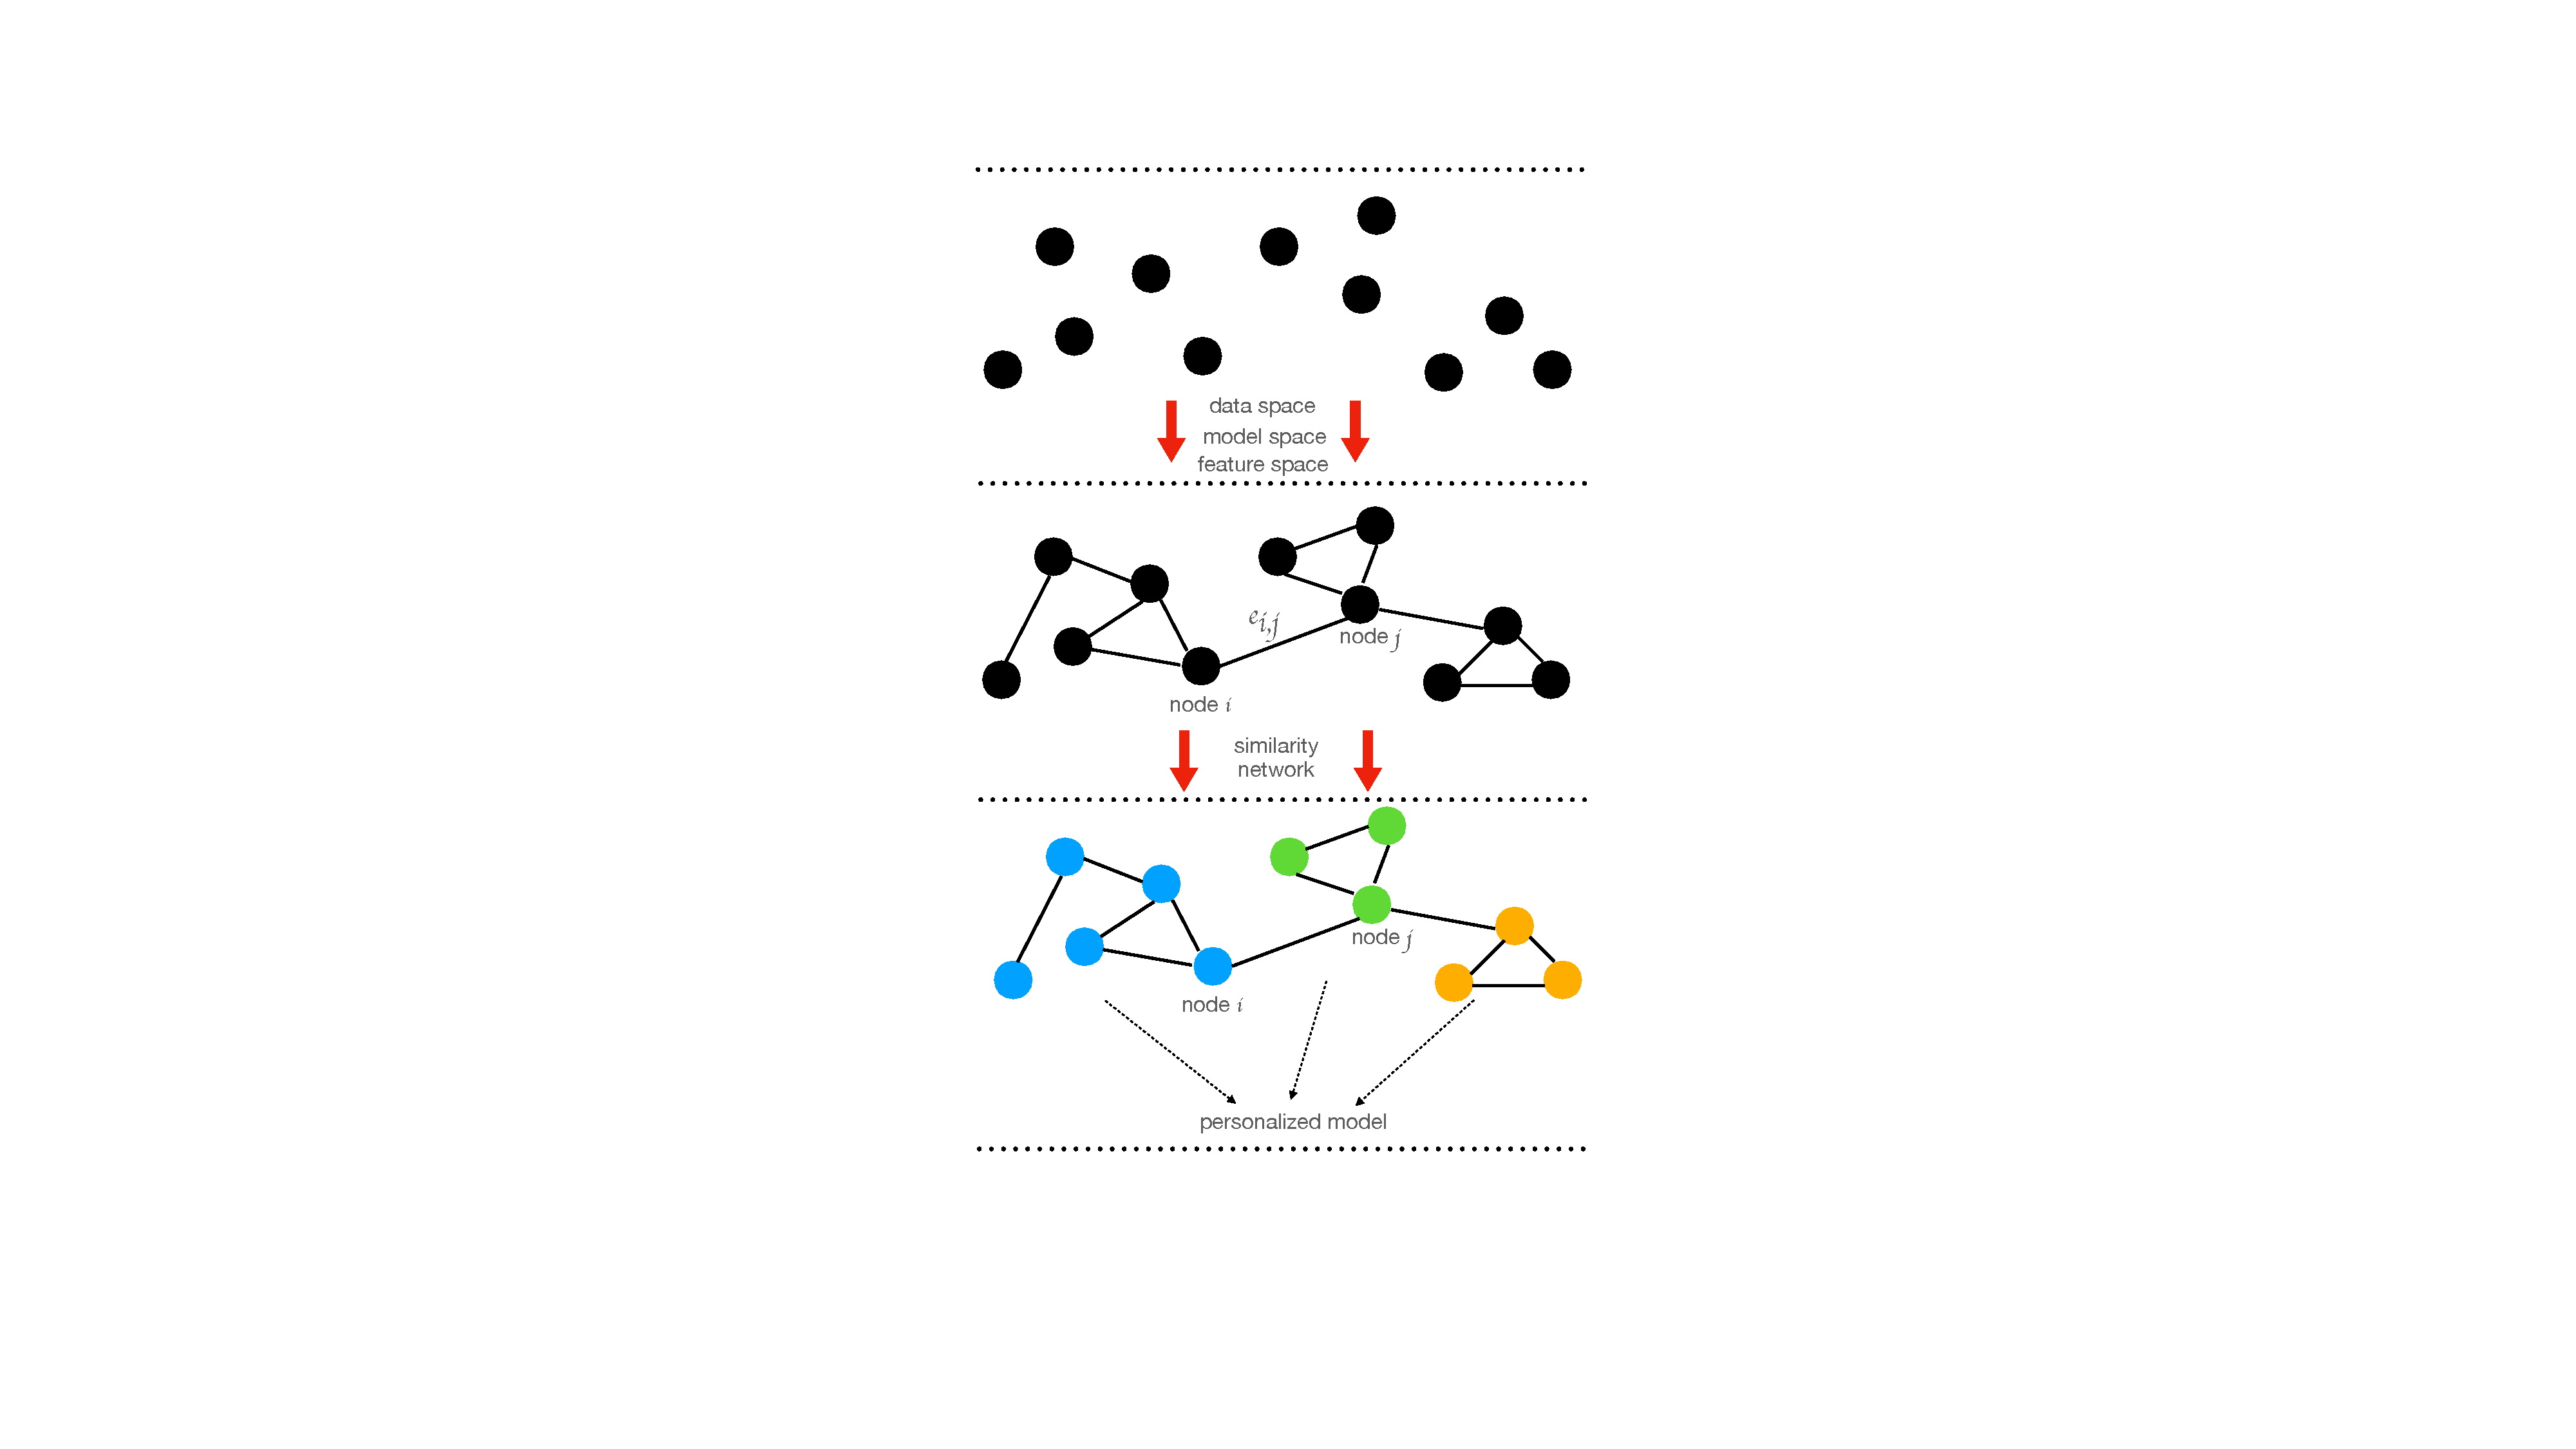
\includegraphics[width=0.97\columnwidth]{figs/figs_networkG}
\caption{Personalized representation based on similarity network}
\label{figure_xxx}
\end{figure}



\subsection{Final Formulation}
Given the mapping matrix $\M\in\RR^{d\times d_1}$ and $\N\in\RR^{d\times d_2}$, the objective problem is formulated by
\begin{align}
\nonumber
\min_{\substack{\{\x^{(n)}\}_{n=1}^N}} \frac{1}{N}\sum_{n\in\Ncal} f_n\lrincir{\x^{(n)}; \Dcal_n} + \lambda \sum_{\substack{e_{i,j} \in \Ecal,\\ \forall i,j\in\Ncal}} \lrnorm{\z^{(i)} - \z^{(j)}}_p,
\end{align} subject to:
\begin{align}
\nonumber
\x^{(n)} = \M\x + \N \z^{(n)},{~~~~}\forall n\in\Ncal, \x\in\RR^{d_1}, \z^{(n)}\in\RR^{d_2}.
\end{align} Here, $p\in\{1,2,\infty\}$. $\M$ and $\N$ has special structure, where every row of them has at most one non-zero value, and the non-zero value is $1$.  

The formulation can be equally transformed as follows.
\begin{align}
\min_{\substack{\{\x^{(n)}\}_{n=1}^N}} \frac{1}{N}\sum_{n=1}^N f_n\lrincir{\x^{(n)}; \Dcal_n} + \lambda \lrnorm{\Z\Q}_{1,p},
\end{align} subject to:
\begin{align}
\x^{(n)} = \M\x + \N \z^{(n)}.
\end{align} Here, $\Z\in\RR^{d_2 \times N}$, $\Q\in\RR^{N\times M}$. $N$ and $M$ represent the total number of nodes and edges in the network $\Gcal$, respectively. 
$\Z$ represents some a variable matrix, consisting of $N$ variables as columns, that is, $\Z = \left [\z^{(1)}, \z^{(2)}, ..., \z^{(N)} \right ]$. $\Q$ is the given auxiliary matrix, which has $M$ columns and every column has two non-zero values: $1$ and $-1$. Note that $\lrnorm{\cdot}_{1,p}$ is denoted by $\ell_{1,p}$ norm. Given a matrix $\U\in\RR^{d_2 \times M}$, it is defined by 
\begin{align}
\nonumber
\lrnorm{\U}_{1,p} := \sum_{m=1}^M \lrnorm{\U_{:, m}}_p.
\end{align}

\begin{figure}[!t]
\setlength{\abovecaptionskip}{0pt}
\setlength{\belowcaptionskip}{0pt}
\centering 
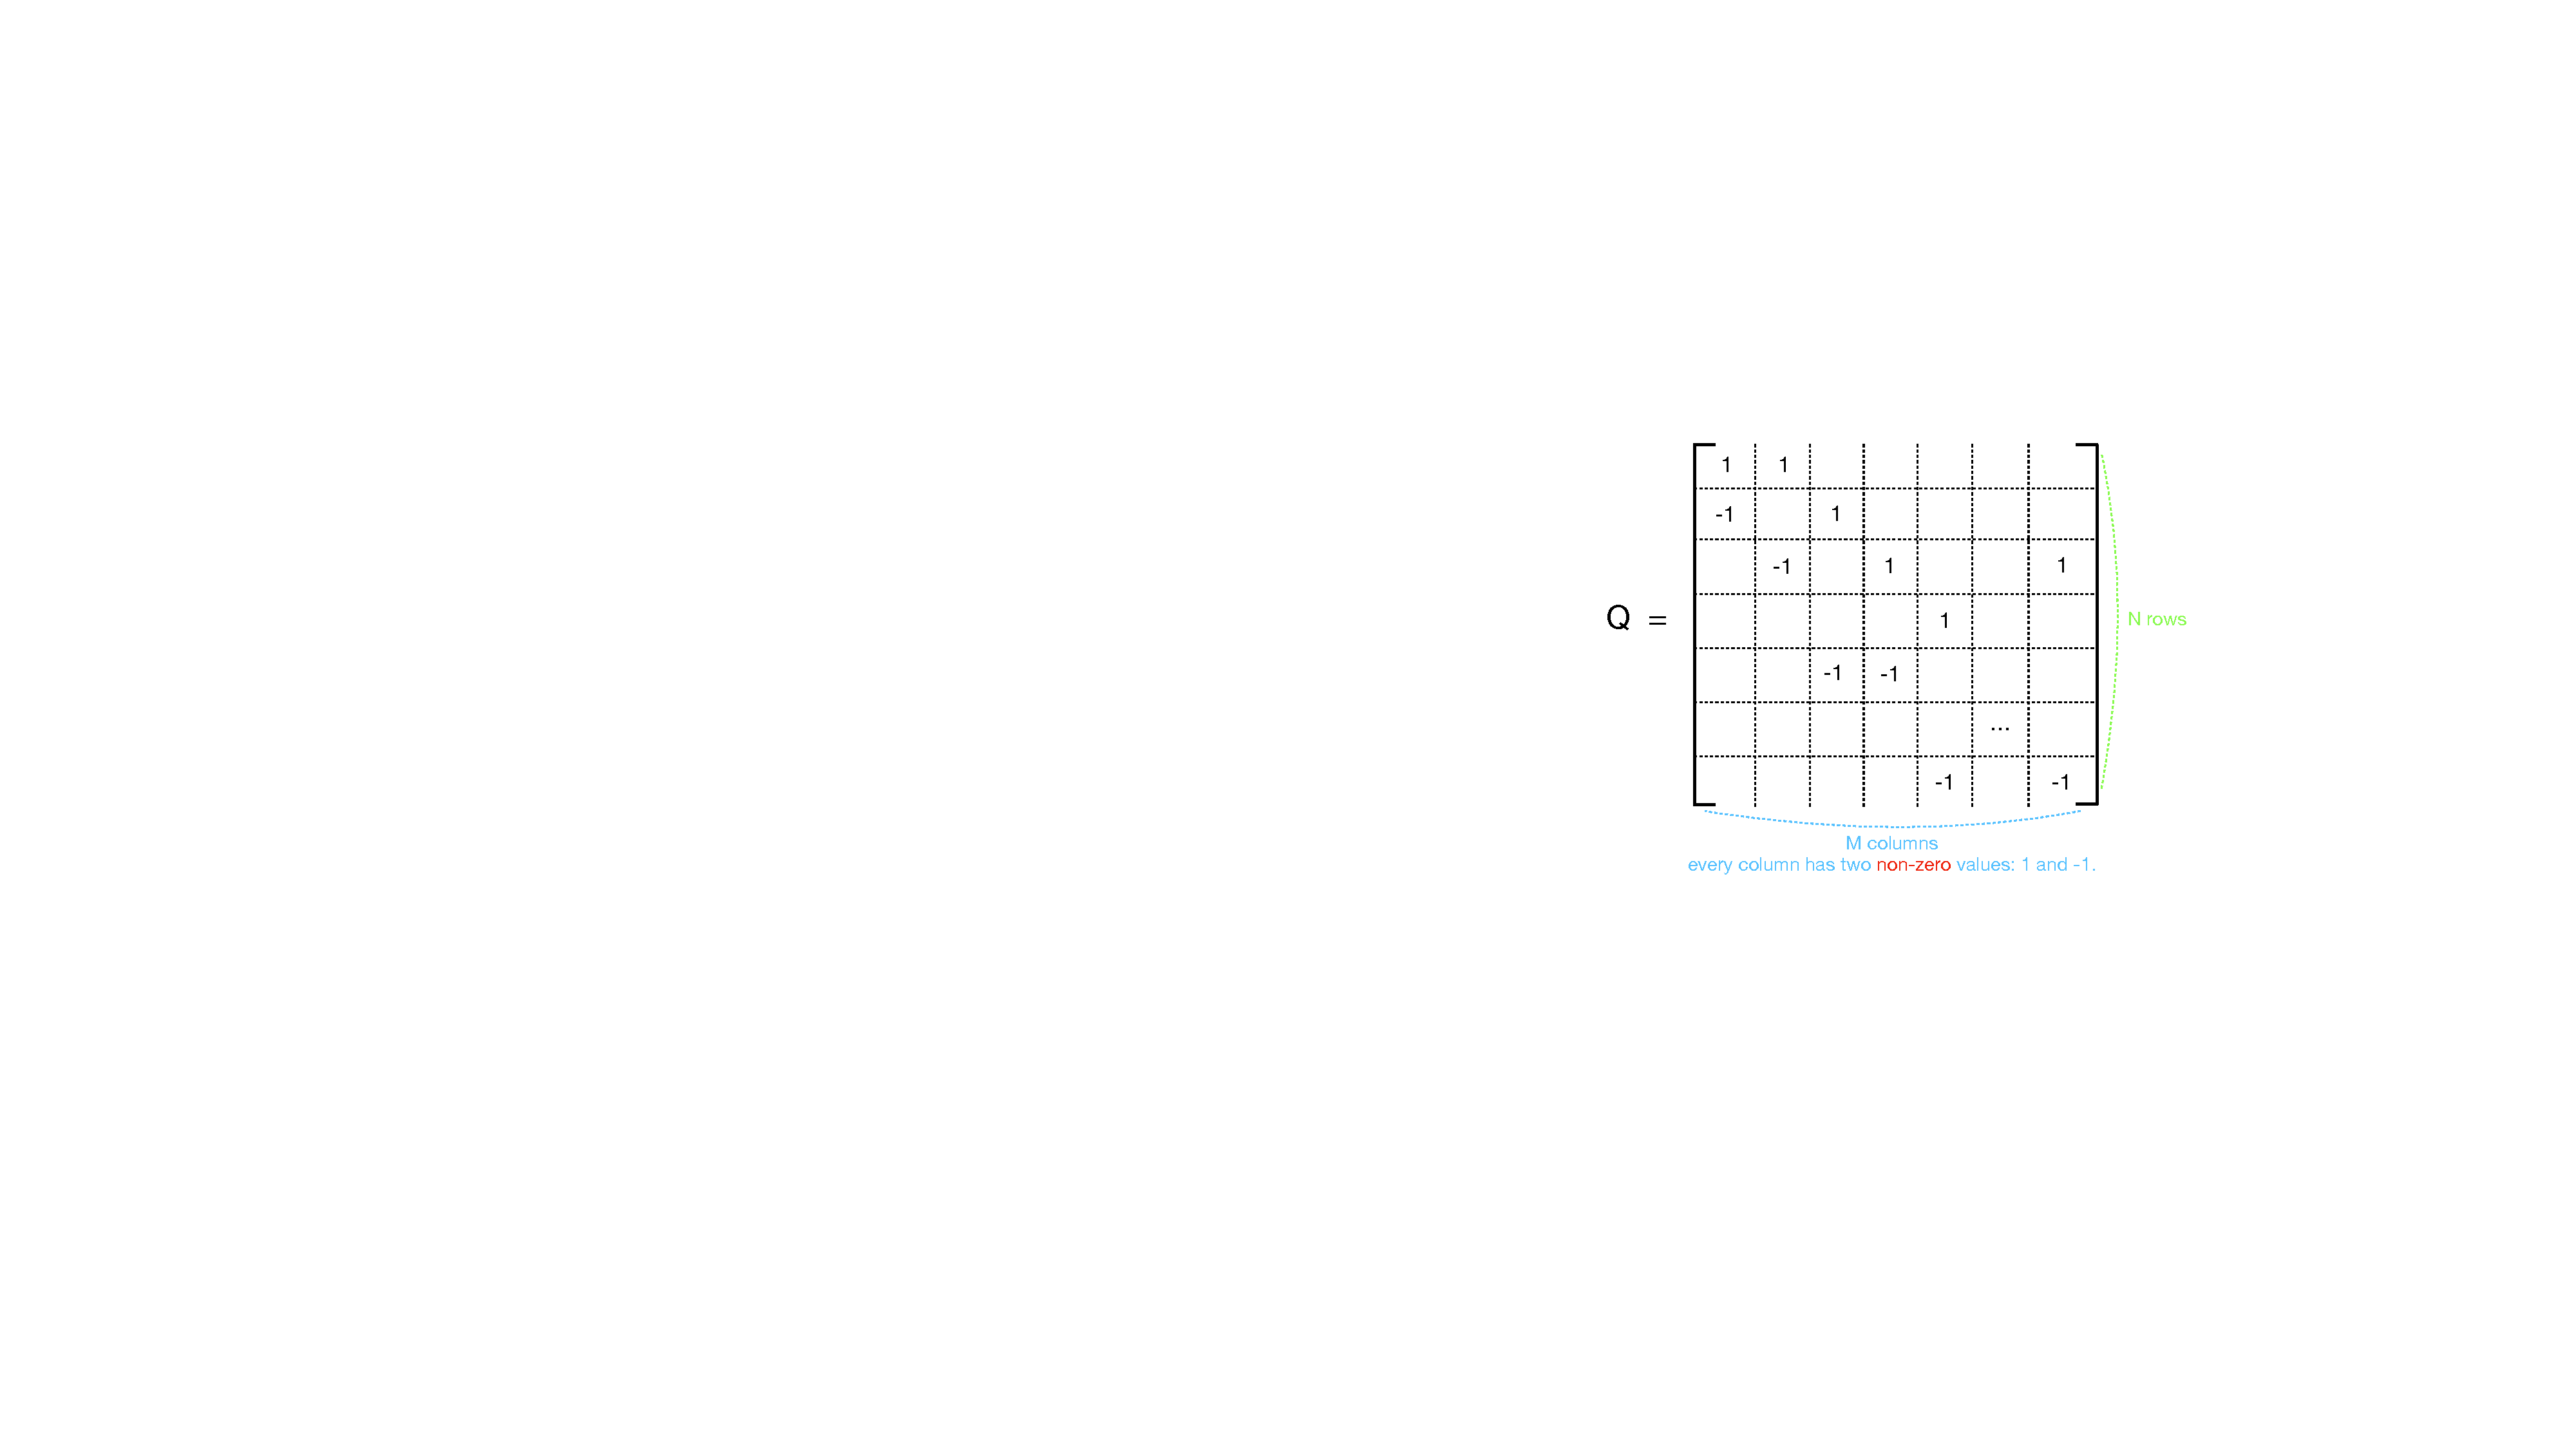
\includegraphics[width=0.97\columnwidth]{figs/figs_Q_matrix}
\caption{$\Q$ matrix.}
\label{figure_xxx}
\end{figure}


\begin{figure}[!t]
\setlength{\abovecaptionskip}{0pt}
\setlength{\belowcaptionskip}{0pt}
\centering 
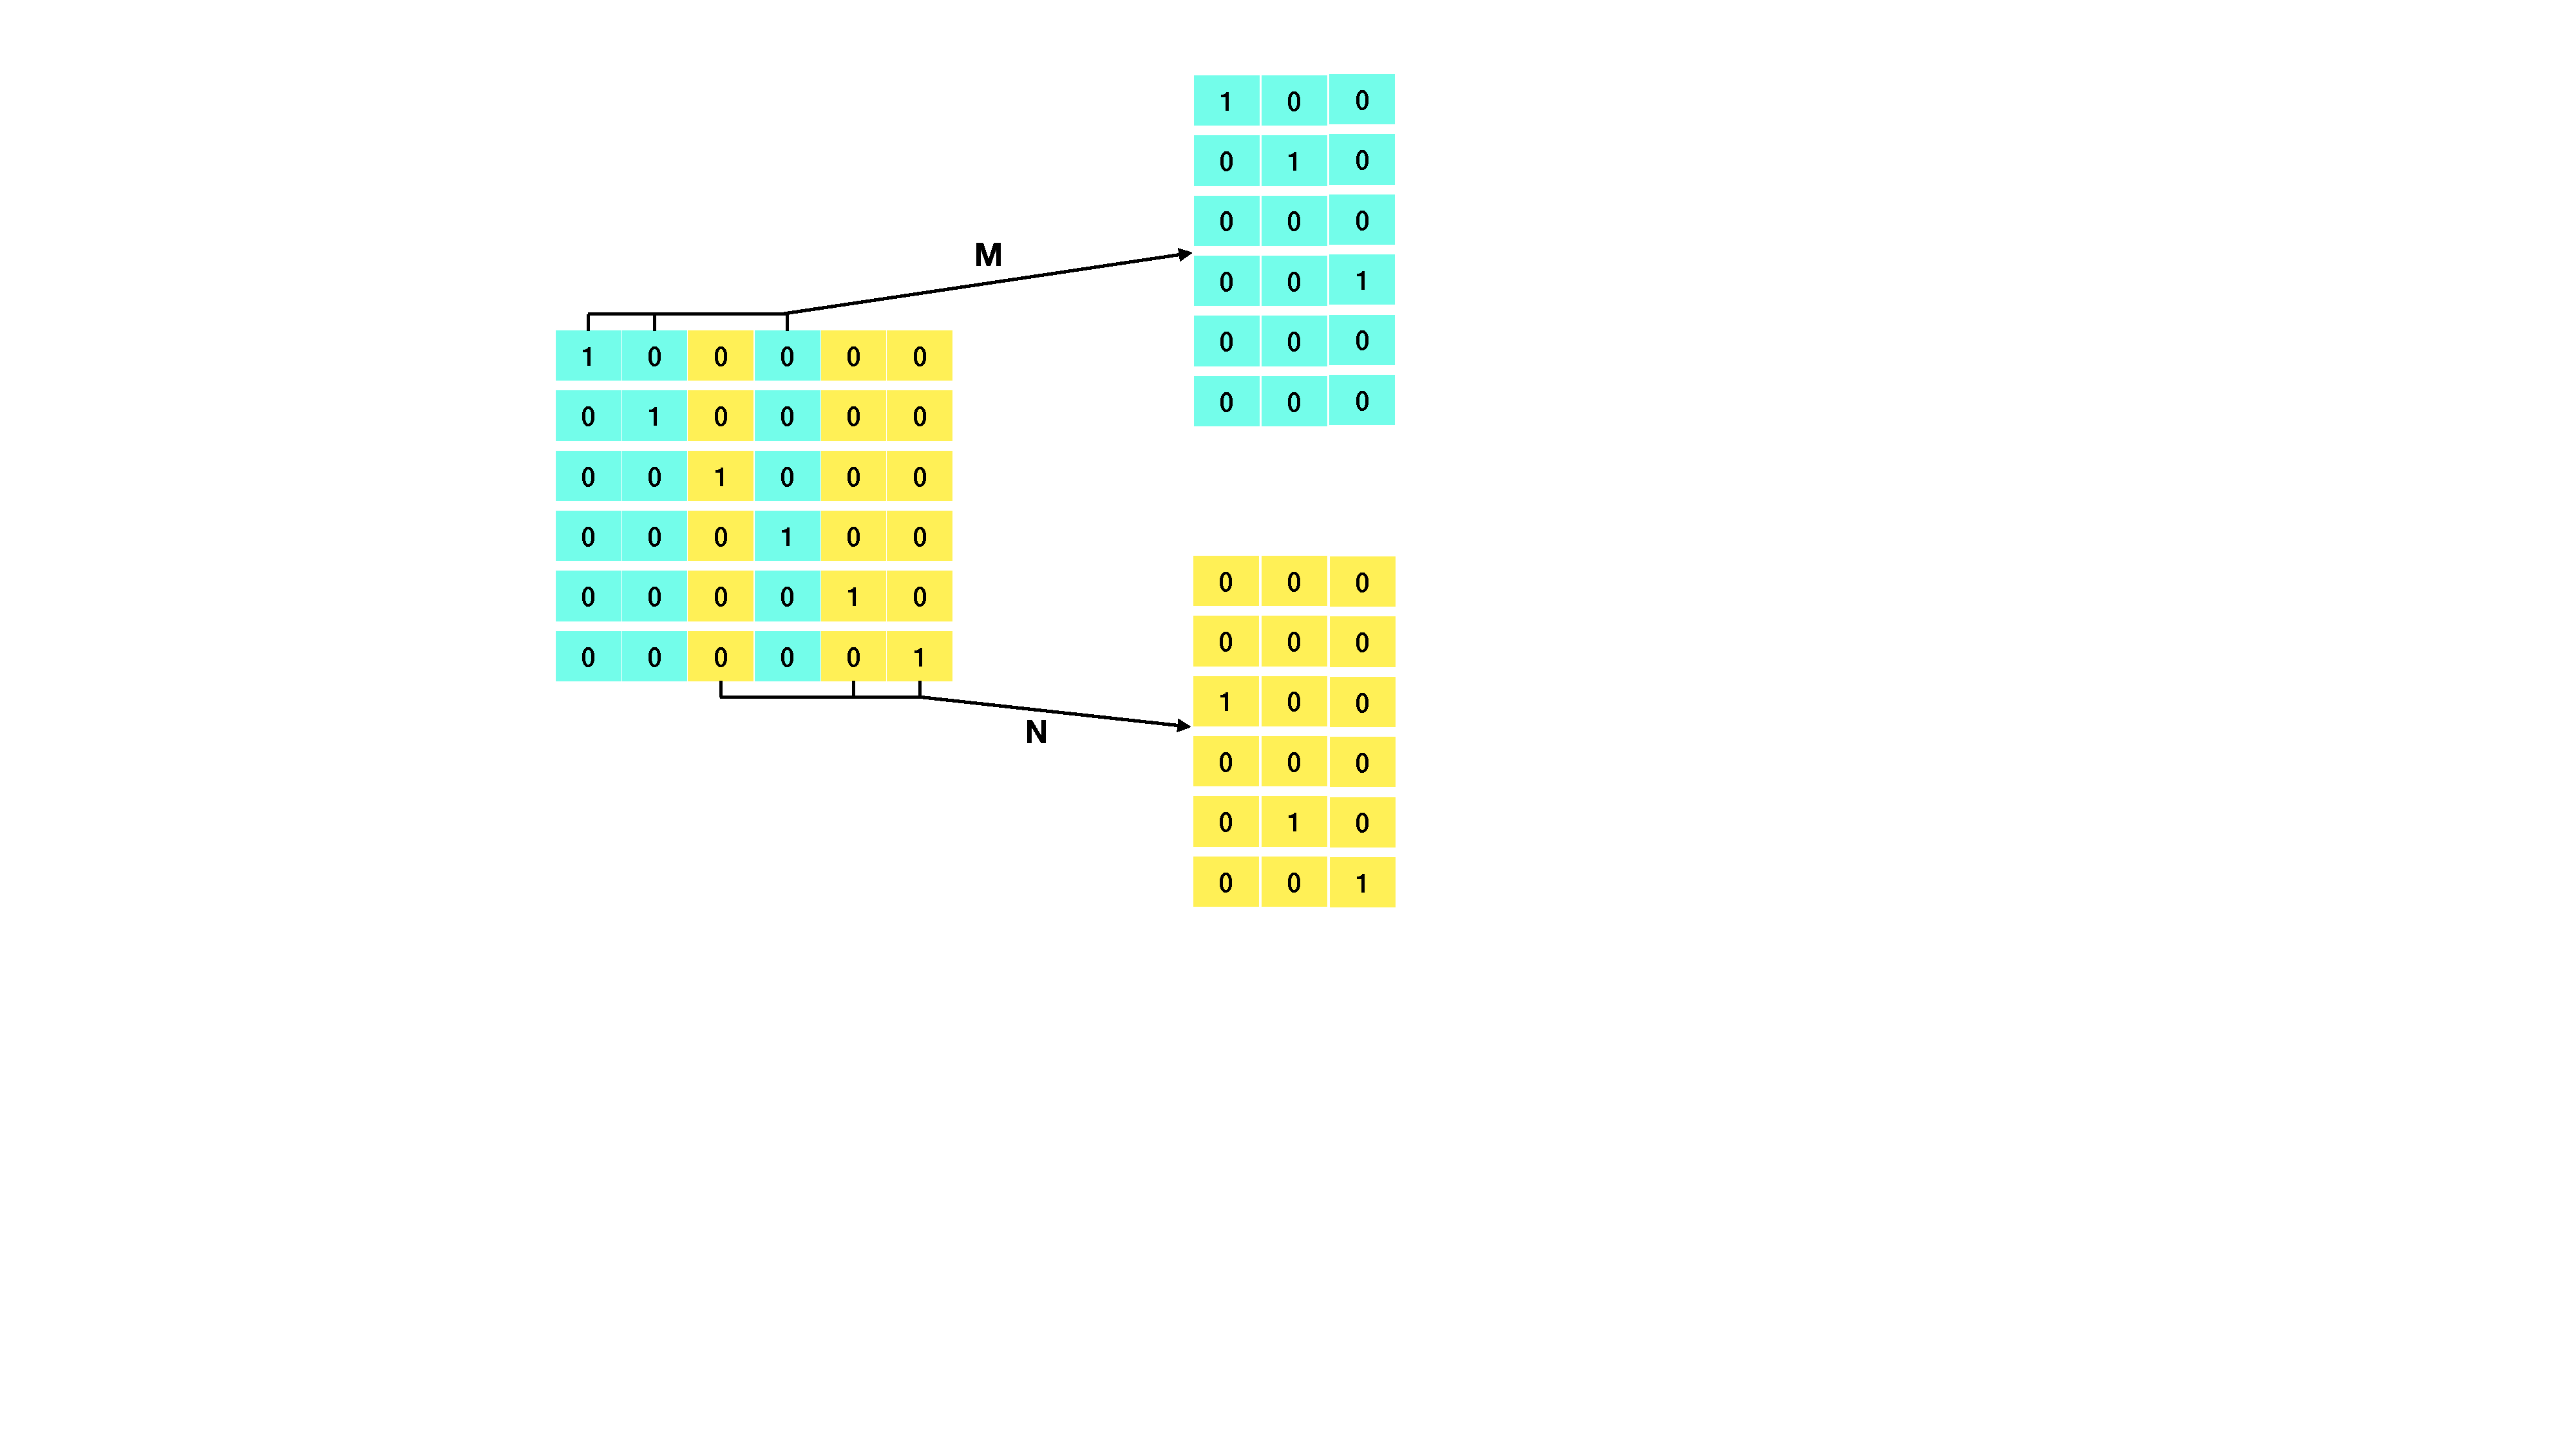
\includegraphics[width=0.97\columnwidth]{figs/figs_MNmatrix}
\caption{for example: $\M$ and $\N$ }
\label{figure_xxx}
\end{figure}


\subsection{Optimization via Alternative method}

\begin{align}
\min_{\substack{\{\x^{(n)}\}_{n=1}^N}} \frac{1}{N}\sum_{n=1}^N f_n\lrincir{\x^{(n)}; \Dcal_n} + \lambda \lrnorm{\Z\Q}_{1,p},
\end{align} subject to:
\begin{align}
\x^{(n)} = \M\x + \N \z^{(n)}.
\end{align}
The variable $\{\x^{(1)}, \x^{(2)}, ..., \x^{(N)}\}$ is obtained by alternatively optimizing $\x$ and $\{\z^{(1)}, \z^{(2)}, ..., \z^{(N)}\}$.

\textbf{Optimizing $\x$ by given $\Z$.} $\x$ is optimized by solving the following problem.
\begin{align}
\min_{\substack{\x\in\RR^{d_1}}} \frac{1}{N}\sum_{n=1}^N f_n\lrincir{\M\x + \N \z^{(n)}; \Dcal_n}.
\end{align} By using the data-driven stochastic optimization method \cite{dd}, we need to perform the following problem to obtain $\x$, iteratively.
\begin{align}
\nonumber
\min_{\substack{\x\in\RR^{d_1}}} \frac{1}{N}\sum_{n=1}^N \lrangle{\M^{-1}\g_t^{(n)}, \x} + \frac{1}{2\eta_t}\lrnorm{\x - \x_t}^2,
\end{align} where $\g_t^{(n)}$ is a stochastic gradient of $f_n$ with $\M\x + \N \z_t^{(n)}$ by using data drawn from the local dataset $\Dcal_n$.


\textbf{Optimizing $\Z$ by given $\x$.}

\begin{align}
\min_{\substack{\Z\in\RR^{d_2\times N}}} \frac{1}{N}\sum_{n=1}^N f_n\lrincir{\M\x + \N \z^{(n)}; \Dcal_n} + \lambda \lrnorm{\Z\Q}_{1,p}.
\end{align}  By using the data-driven stochastic optimization method \cite{dd}, we need to perform the following problem.
\begin{align}
\nonumber
\min_{\substack{\Z\in\RR^{d_2\times N}}} \frac{1}{N}\sum_{n=1}^N \lrangle{\N^{-1} \g_t^{(n)}, \z^{(n)}} + \lambda \lrnorm{\Z\Q}_{1,p} + \frac{1}{2\eta_t}\lrnorm{\Z - \Z_t}_F^2.
\end{align} $\g_t^{(n)}$ is a stochastic gradient of $f_n$ with $\M\x_t + \N \z^{(n)}$ by using stochastic data  drawn from the local dataset $\Dcal_n$. Suppose $\G_t = \left [ \g_t^{(1)}, \g_t^{(2)}, ..., \g_t^{(N)} \right ]$, $\Z$ is optimized by performing the following problem.
\begin{align}
\nonumber
\min_{\substack{\Z\in\RR^{d_2\times N}}} \frac{1}{N}\1_d^\top\lrincir{\G_t \odot \Z}\1_N + \lambda \lrnorm{\Z\Q}_{1,p} + \frac{1}{2\eta_t}\lrnorm{\Z - \Z_t}_F^2.
\end{align}

\textbf{On client.}  

\begin{algorithm}[!]
    \caption{Compute local stochastic gradient at the $n$-th client for the $t+1$-th iteration.}
    \label{algo_xxx}
    \begin{algorithmic}[1]
        %\Require The number of total iterations $T$, and the initial parameter $\x_1$.
        %\algotext{\textbf{On the $n$-th client for the $t+1$-th iteration:}}
        \State Receive the parameter $\y_t^{(n)} := \M\x_t + \N\z_t^{(n)}$ from the server.
        \State Randomly sample an instance $\a\sim\Dcal_n$, and compute the stochastic gradient $\g^{(n)}_t = \nabla f(\y_t^{(n)};\a)$ with $\a\sim\Dcal_n$.
        \State Send $\g^{(n)}_t$ to the server.
    \end{algorithmic}
\end{algorithm} 





\textbf{On server.}

\begin{algorithm}[!]
    \caption{Training of personalized models on the server.}
    \label{algo_xxx}
    \begin{algorithmic}[1]
        \Require The number of total iterations $T$, and the initial parameter $\x_1$.
        %\algotext{\textbf{On the server:}}
        \State Deliver the parameter $\y_1^{(n)} = \M\x_1 + \N\z_1^{(n)}$ to all client $n$ with $n\in\{1,2, ..., N\}$.
        \For {$t=1,2, ..., T$}
            \State Collect stochastic gradient $\G_t = \left [ \g_t^{(1)}, \g_t^{(2)}, ..., \g_t^{(N)} \right ]$ from all client $n$ with $n\in\{1,2, ..., N\}$.
            \State Update the global parameter $\x$ by performing:
            $$ \x_{t+1} = \argmin_{\substack{\x\in\RR^{d_1}}} \frac{1}{N}\sum_{n=1}^N \lrangle{\M^{-1}\g_t^{(n)}, \x} + \frac{1}{2\eta_t}\lrnorm{\x - \x_t}^2.$$
            \State Update the personalized parameter $\Z$ by performing:
            \begin{align}
            \nonumber
            &\Z_{t+1} \\ \nonumber
            = & \argmin_{\substack{\Z\in\RR^{d_2\times N}}} \frac{\1_d^\top\lrincir{\G_t \odot \Z}\1_N}{N} + \lambda \lrnorm{\Z\Q}_{1,p} + \frac{1}{2\eta_t}\lrnorm{\Z - \Z_t}_F^2.
            \end{align}
            \State Deliver the parameter $\y_{t+1}^{(n)} = \M\x_{t+1} + \N\z_{t+1}^{(n)}$ to every client.
        \EndFor
        \Return $\x_{T+1}^{(n)} = \M\x_{T+1} + \N\z_{T+1}^{(n)}$ with $n\in\{1,2, ..., N\}$.
      \end{algorithmic}
\end{algorithm} 

\subsection{Workflow}


\begin{figure*}[!t]
\setlength{\abovecaptionskip}{0pt}
\setlength{\belowcaptionskip}{0pt}
\centering 
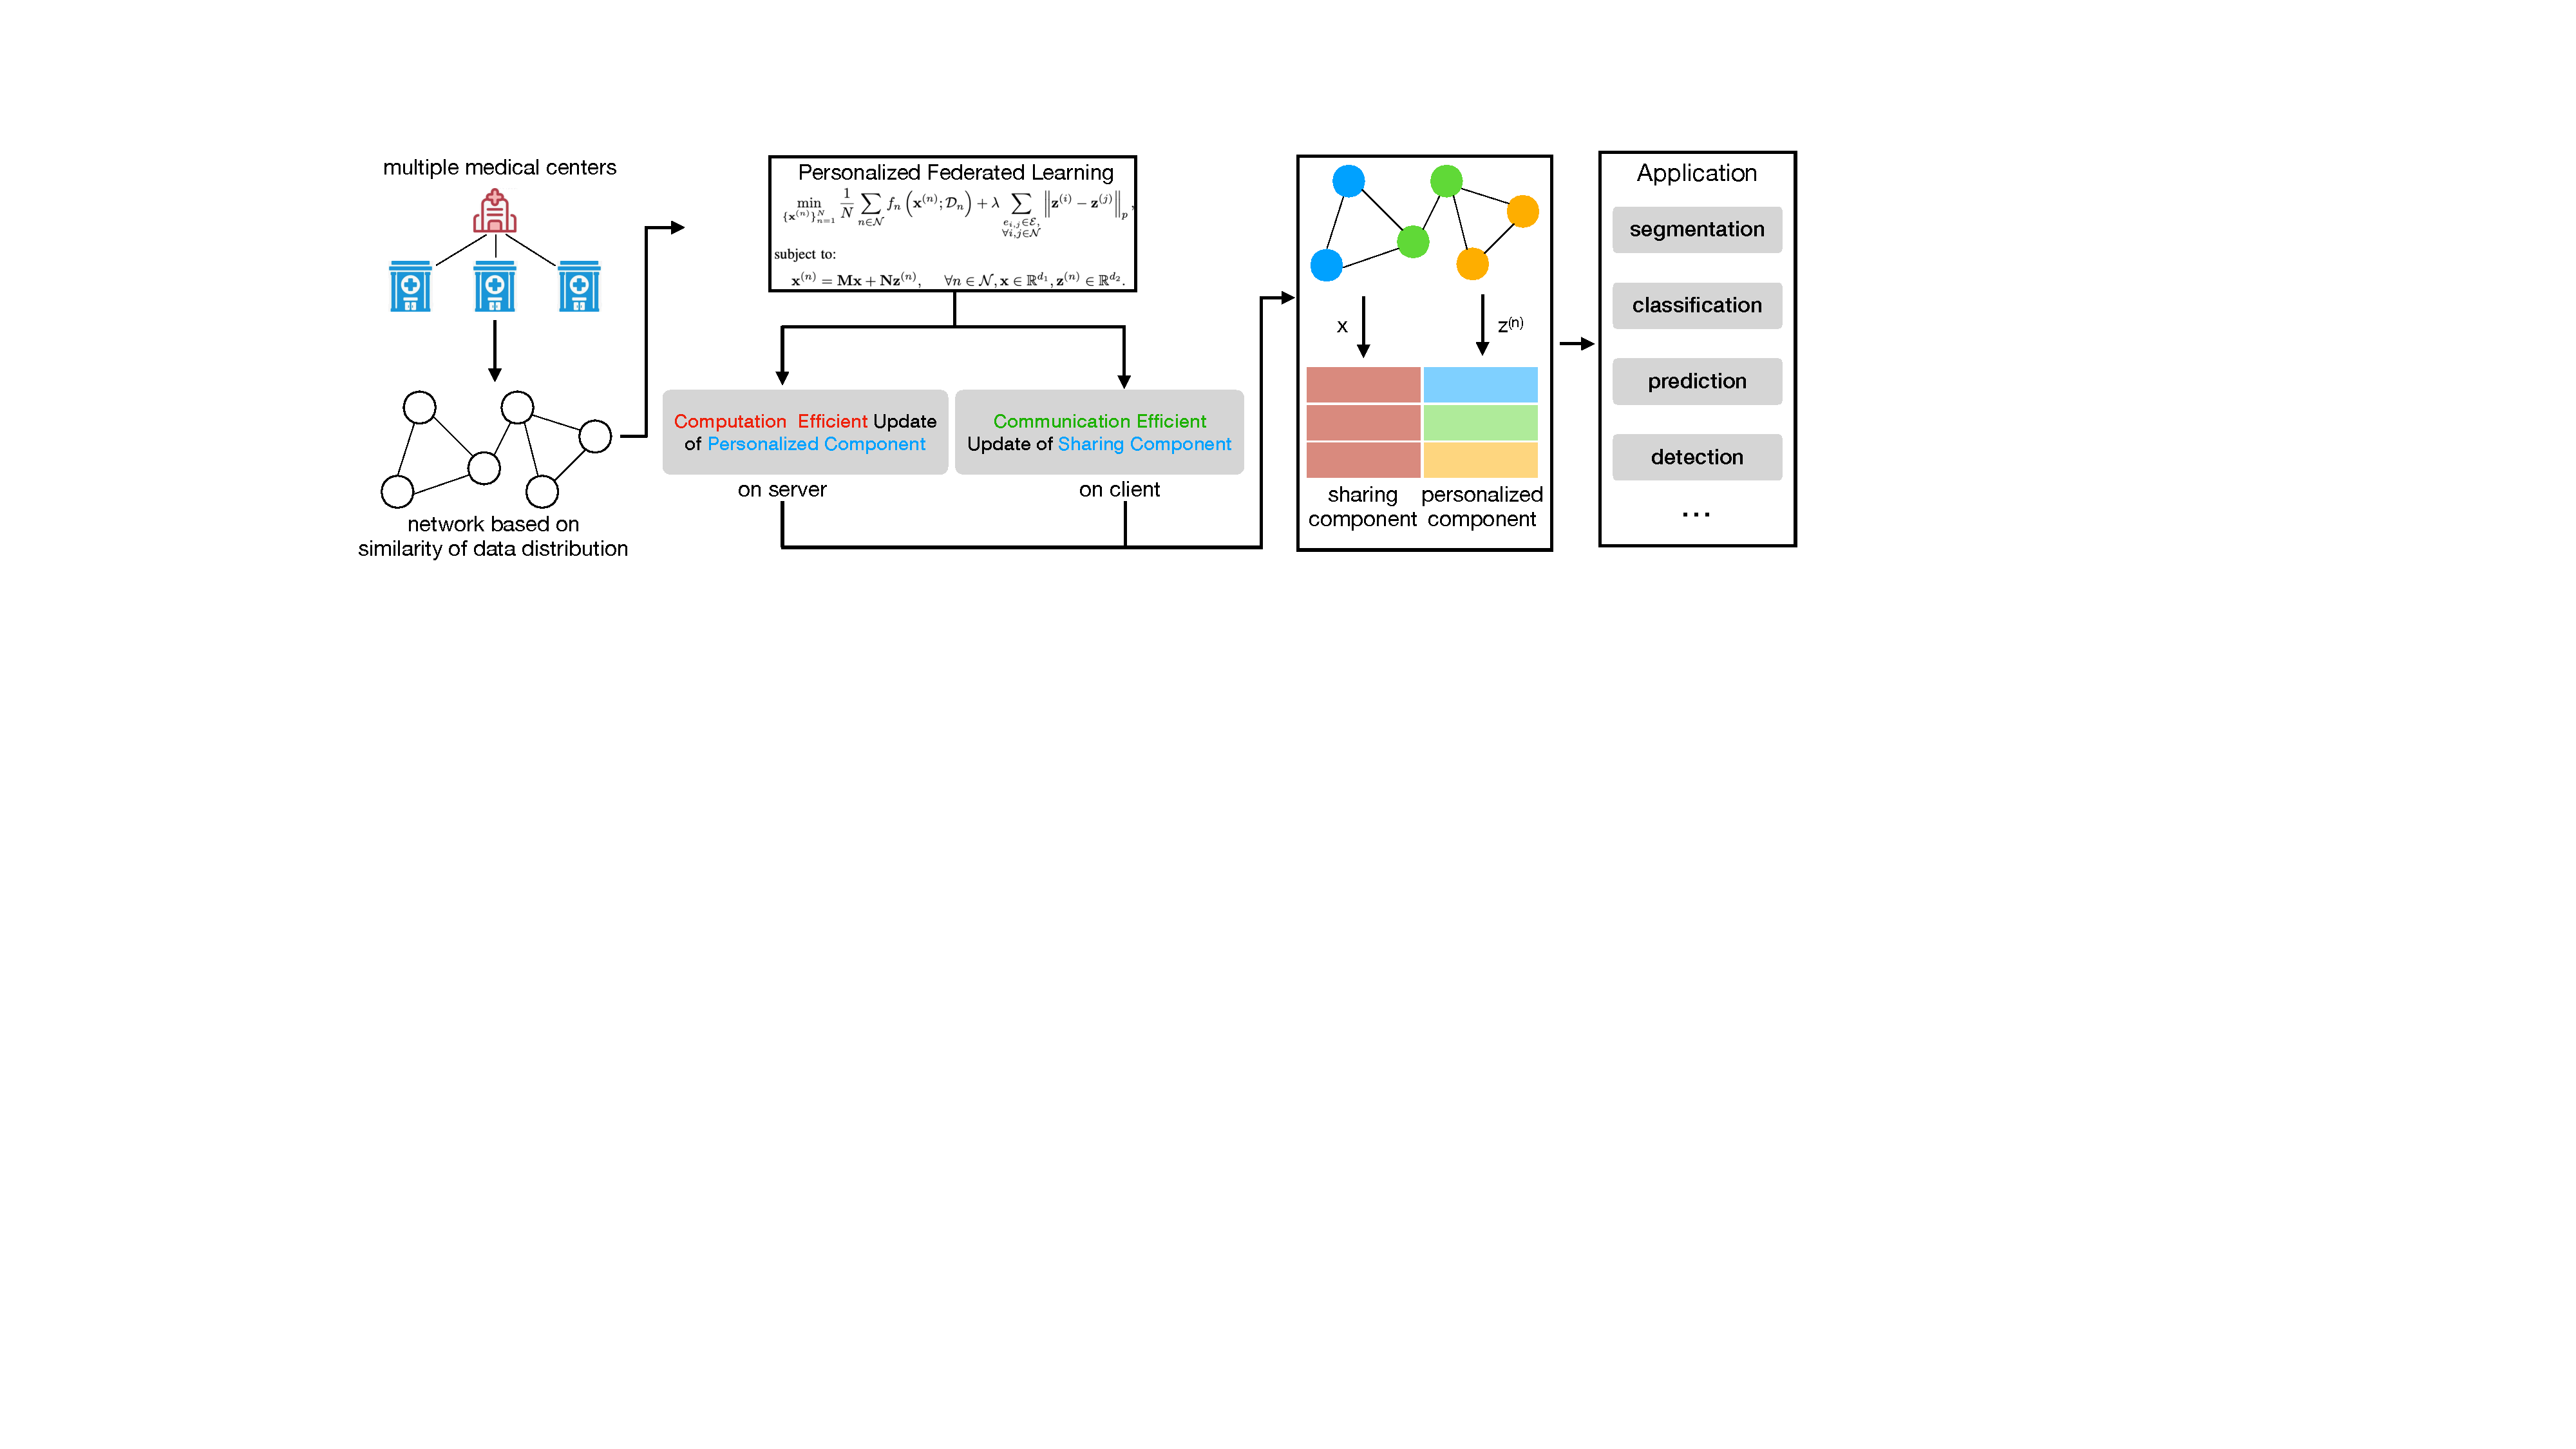
\includegraphics[width=1.98\columnwidth]{figs/figs_workflow}
\caption{workflow}
\label{figure_xxx}
\end{figure*}




\section{Communication Efficient Update of Model}

Recall that stochastic gradient descent is usually used to solve a general optimization problem in the distributed setting, namely Distributed Stochastic Gradient Descent (DSGD). Since every client has to send the update of parameter $\g^{(n)}_t$ to the server, the workload of the network communication  becomes very heavy for a large number of clients. When the workload of the the network communication is heavy, the previous DSGD has to consume much time to complete the data transmission, which impairs the convergence performance of DSGD.  

\subsection{Communication Efficient Regularizer}

In the work, we propose a communication efficient method, which can let $\g_t^{(n)}$ be encoded by using few bits. Since the code length of $\g_t^{(n)}$ is much reduced, the communication efficiency is significantly increased. The basic idea is to induce the cluster structure of elements of $\g_t^{(n)}$ by using differential sparsity regularizer. The regularizer encourages the update of parameter $\nabla_{t+1}^{(n)}$ to own clustering structures. Figure \ref{figure_intro_gradient_clustering} presents an illustrative example. According to Figures \ref{figure_intro_gradient_clustering_without_clustering} and \ref{figure_intro_gradient_clustering_with_clustering},  we observe when the elements of $\nabla_{t+1}^{(n)}$ own clustering structures, they can be encoded by using fewer bits. Its code length can be reduced a lot. The update of parameter can be transmitted from clients  and the server efficiently. According to Figures \ref{figure_intro_gradient_without_clustering_details} and \ref{figure_intro_gradient_with_clustering_details}, our basic idea is to let the difference between the elements of $\nabla_{t+1}^{(n)}$ be sparse, which encourages the elements of $\nabla_{t+1}^{(n)}$ to have clustering structures. Comparing with the gradient quantization methods in the previous studies, the proposed method is able to find a good tradeoff between the convergence performance and the communication efficiency.  It is highlighted that the proposed method does not impair the convergence performance theoretically. 

\begin{figure}[!t]
\setlength{\abovecaptionskip}{0pt}
\setlength{\belowcaptionskip}{0pt}
\centering 
\subfigure[$\nabla_{t+1}^{(n)}$  without clustering structures]{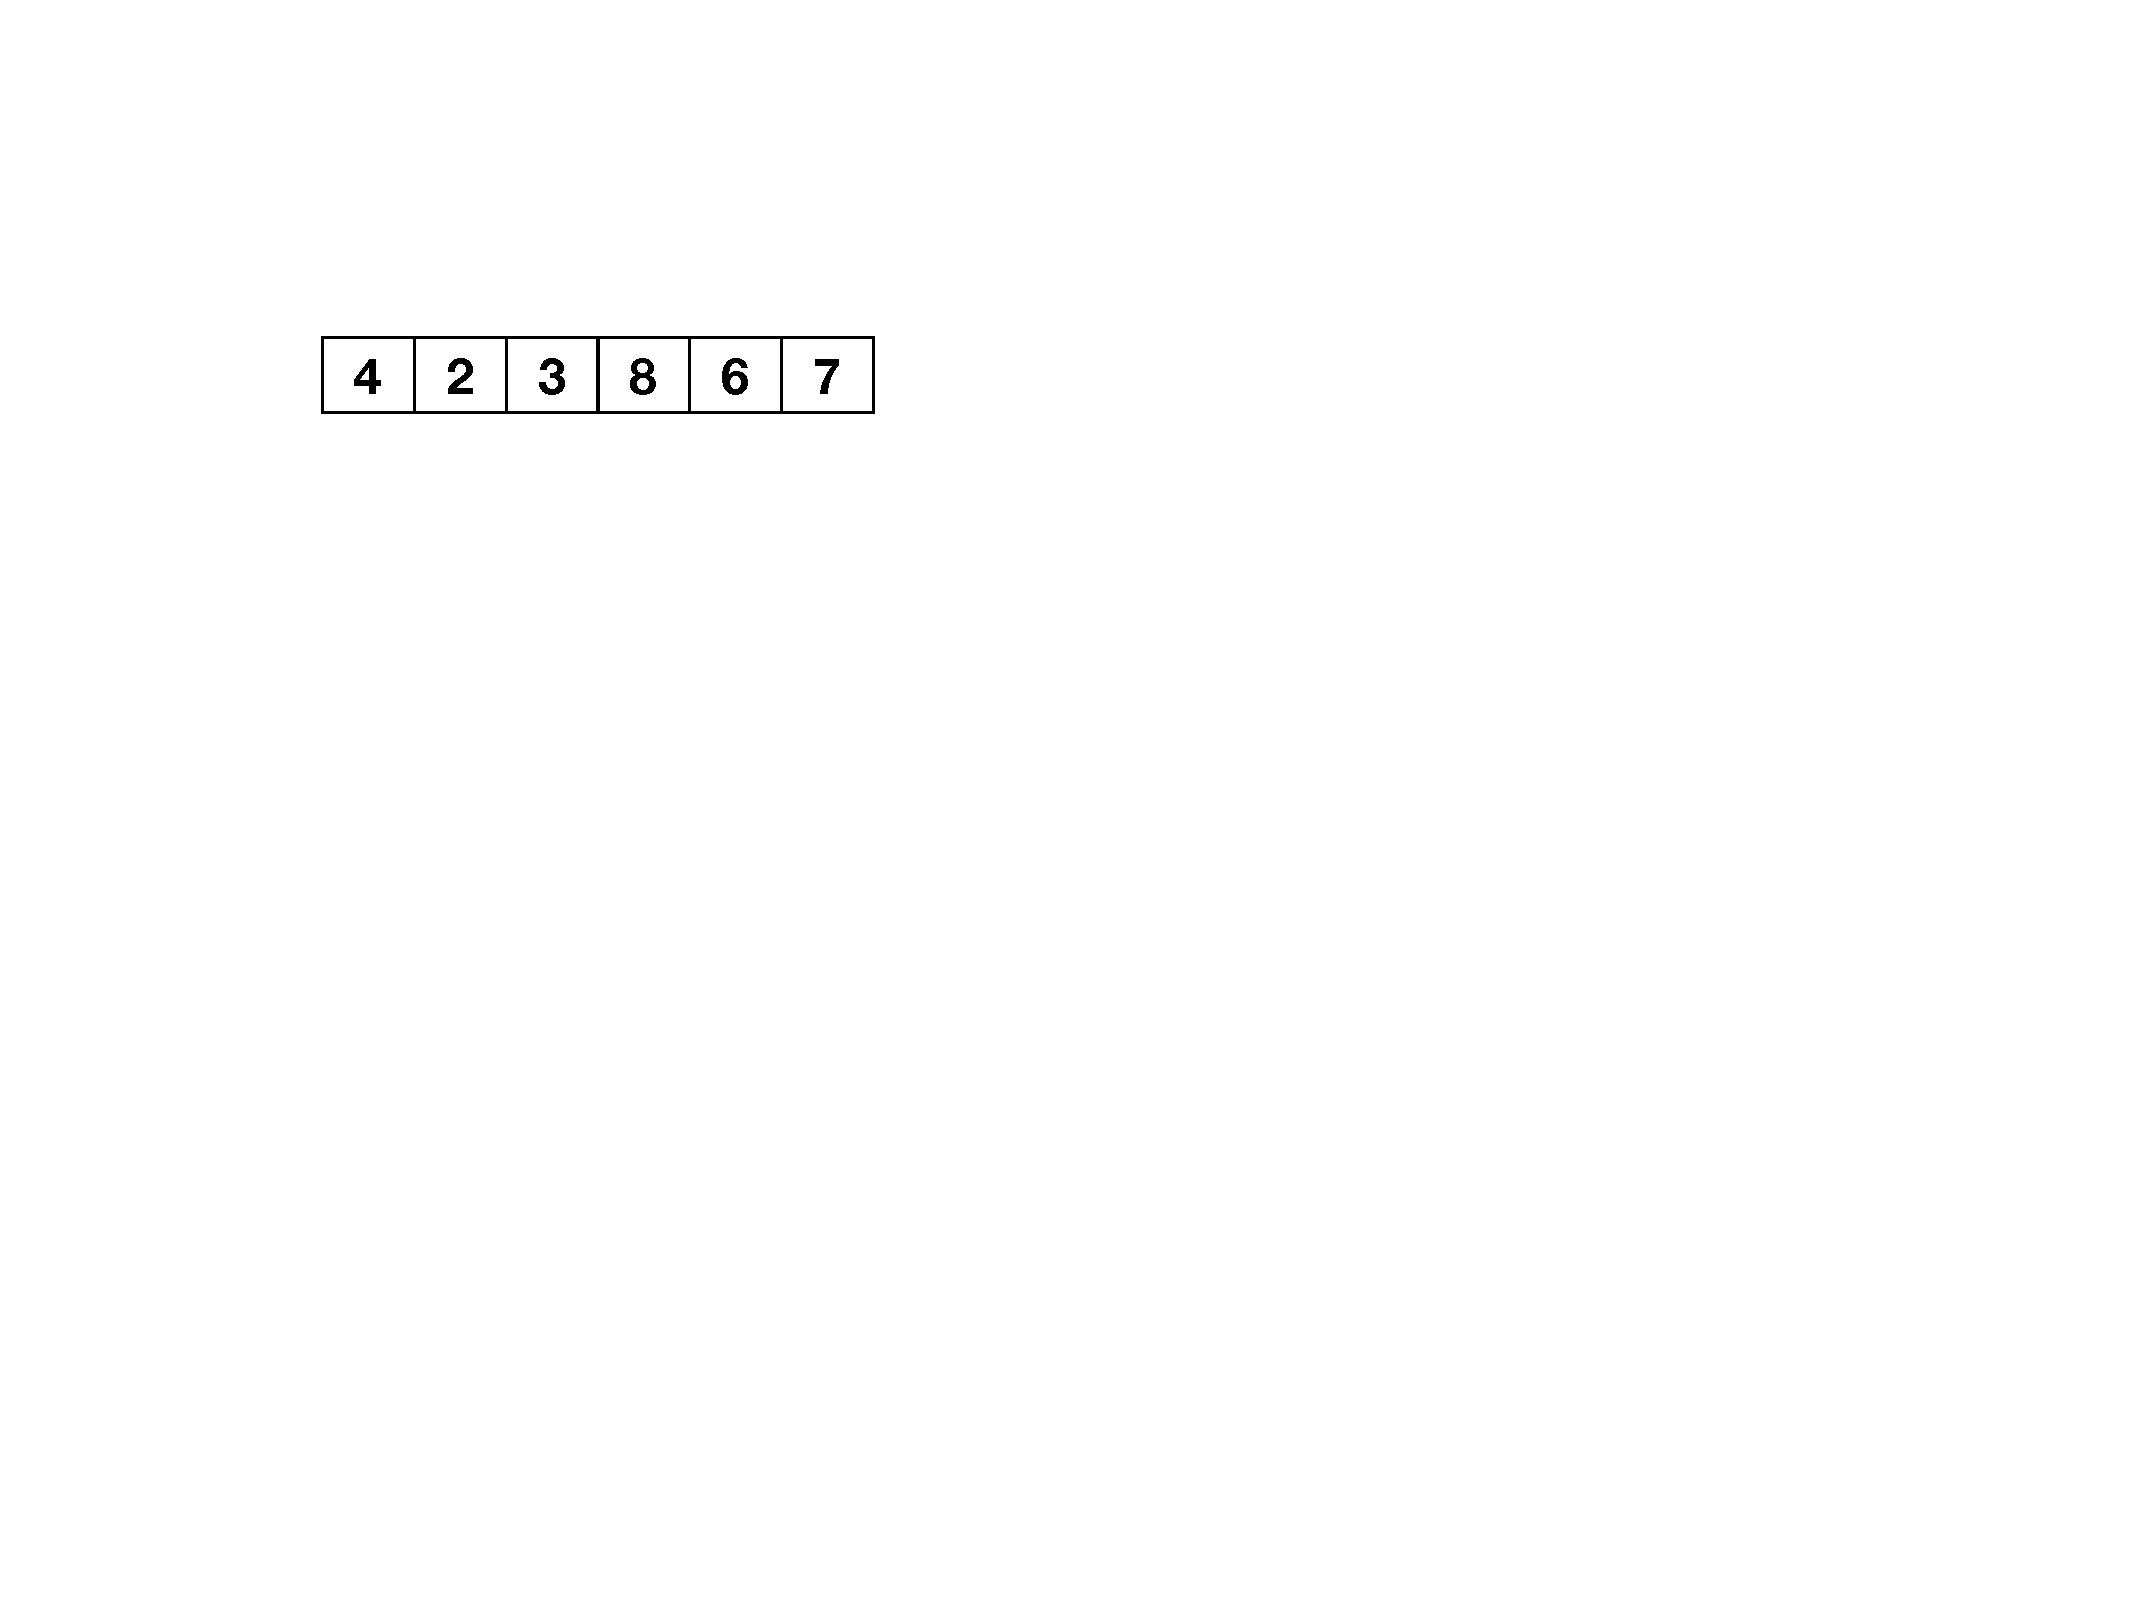
\includegraphics[width=0.48\columnwidth]{figs/figure_intro_gradient_clustering_without_clustering}\label{figure_intro_gradient_clustering_without_clustering}}
\subfigure[Difference between elements of $\nabla_{t+1}^{(n)}$  (without clustering structures) is dense.]{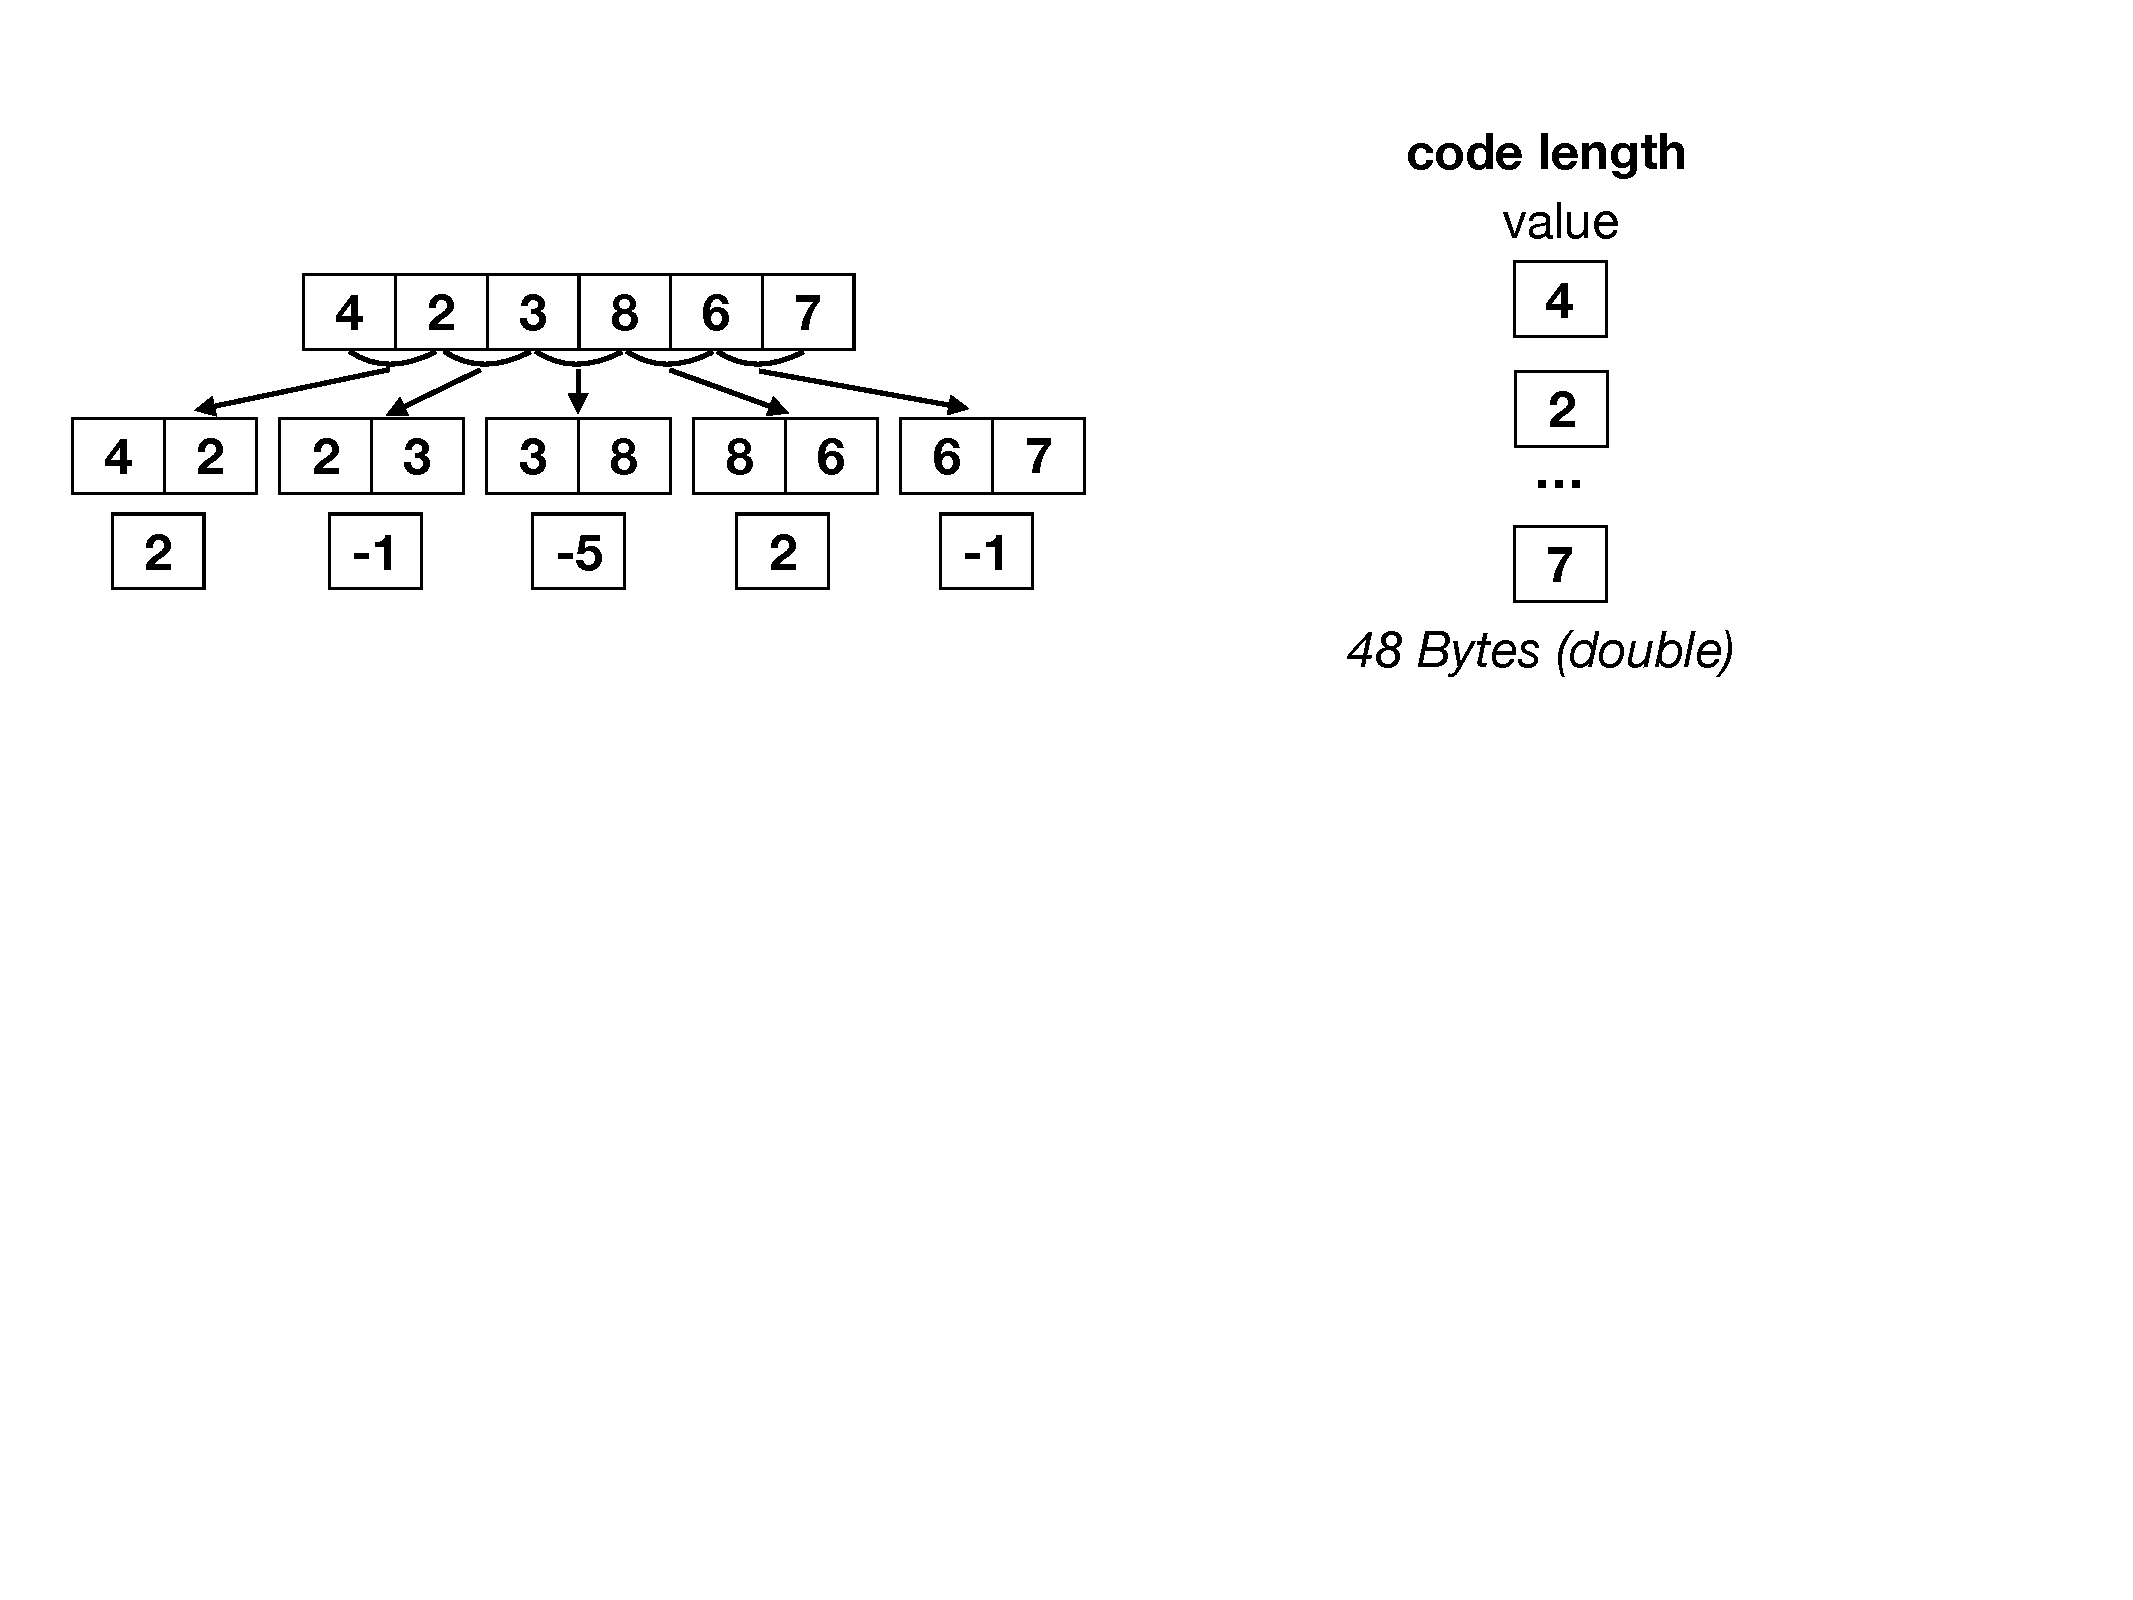
\includegraphics[width=0.9\columnwidth]{figs/figure_intro_gradient_without_clustering_details}\label{figure_intro_gradient_without_clustering_details}}
\subfigure[$\nabla_{t+1}^{(n)}$ with clustering structures]{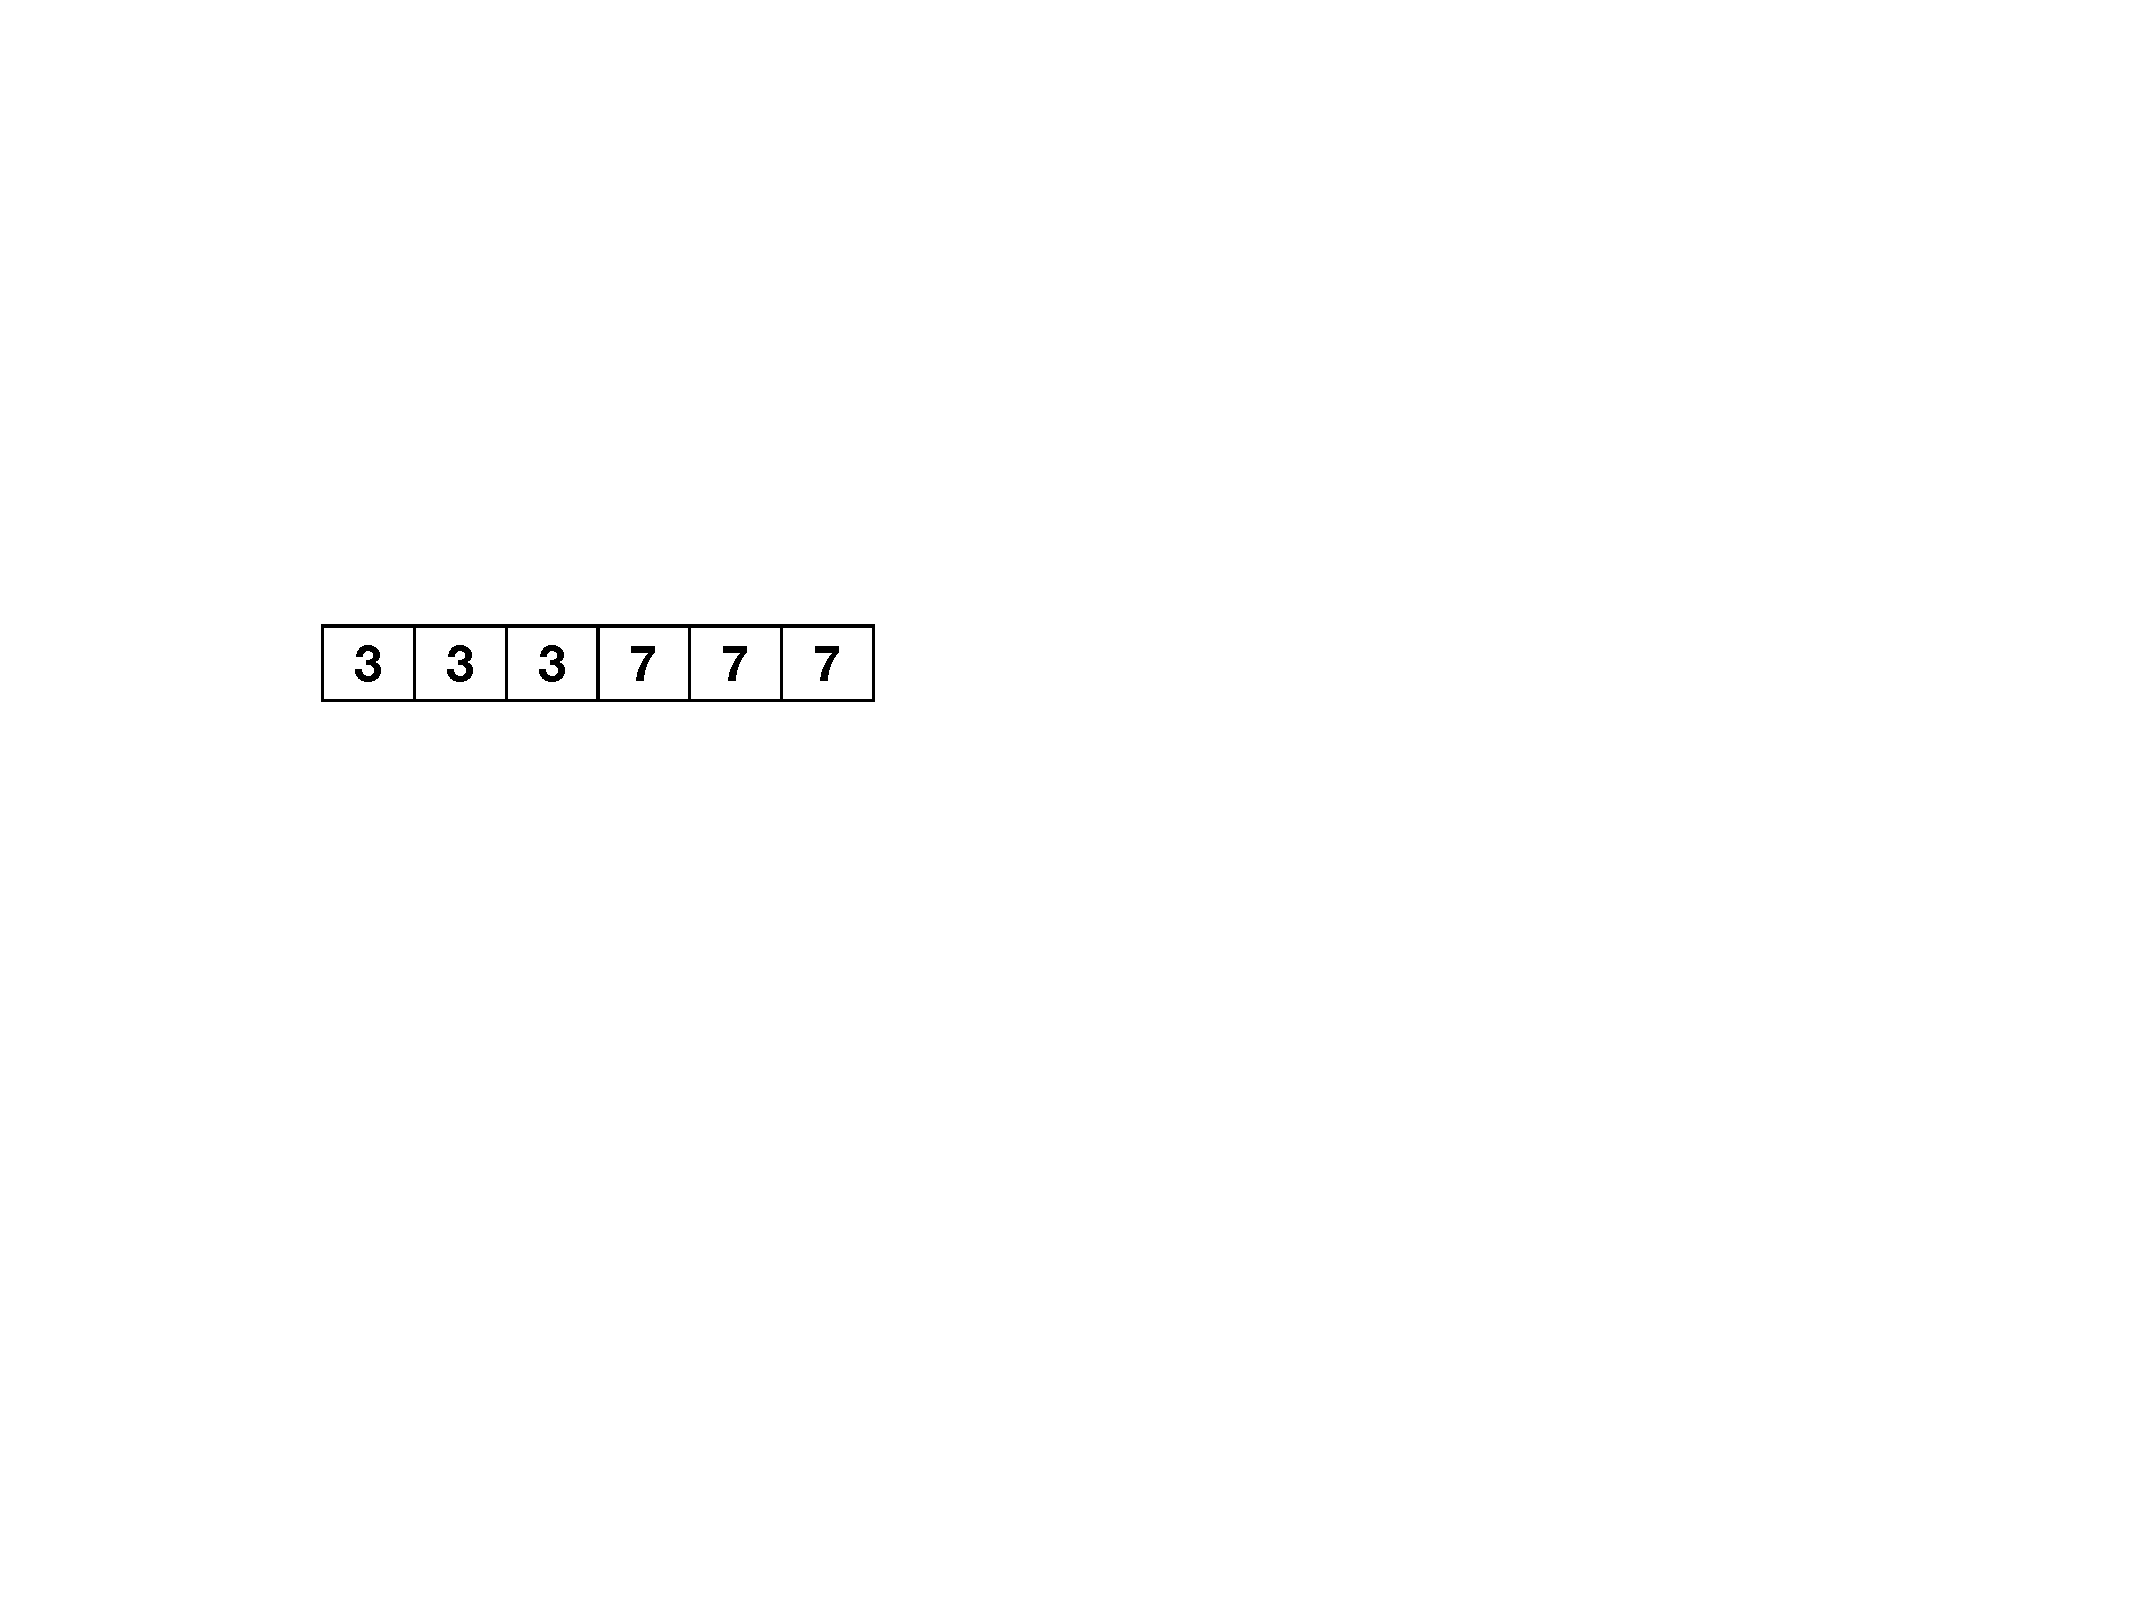
\includegraphics[width=0.48\columnwidth]{figs/figure_intro_gradient_clustering_with_clustering}\label{figure_intro_gradient_clustering_with_clustering}}
\subfigure[Difference between elements of $\nabla_{t+1}^{(n)}$  (with clustering structures) is \textbf{sparse}.]{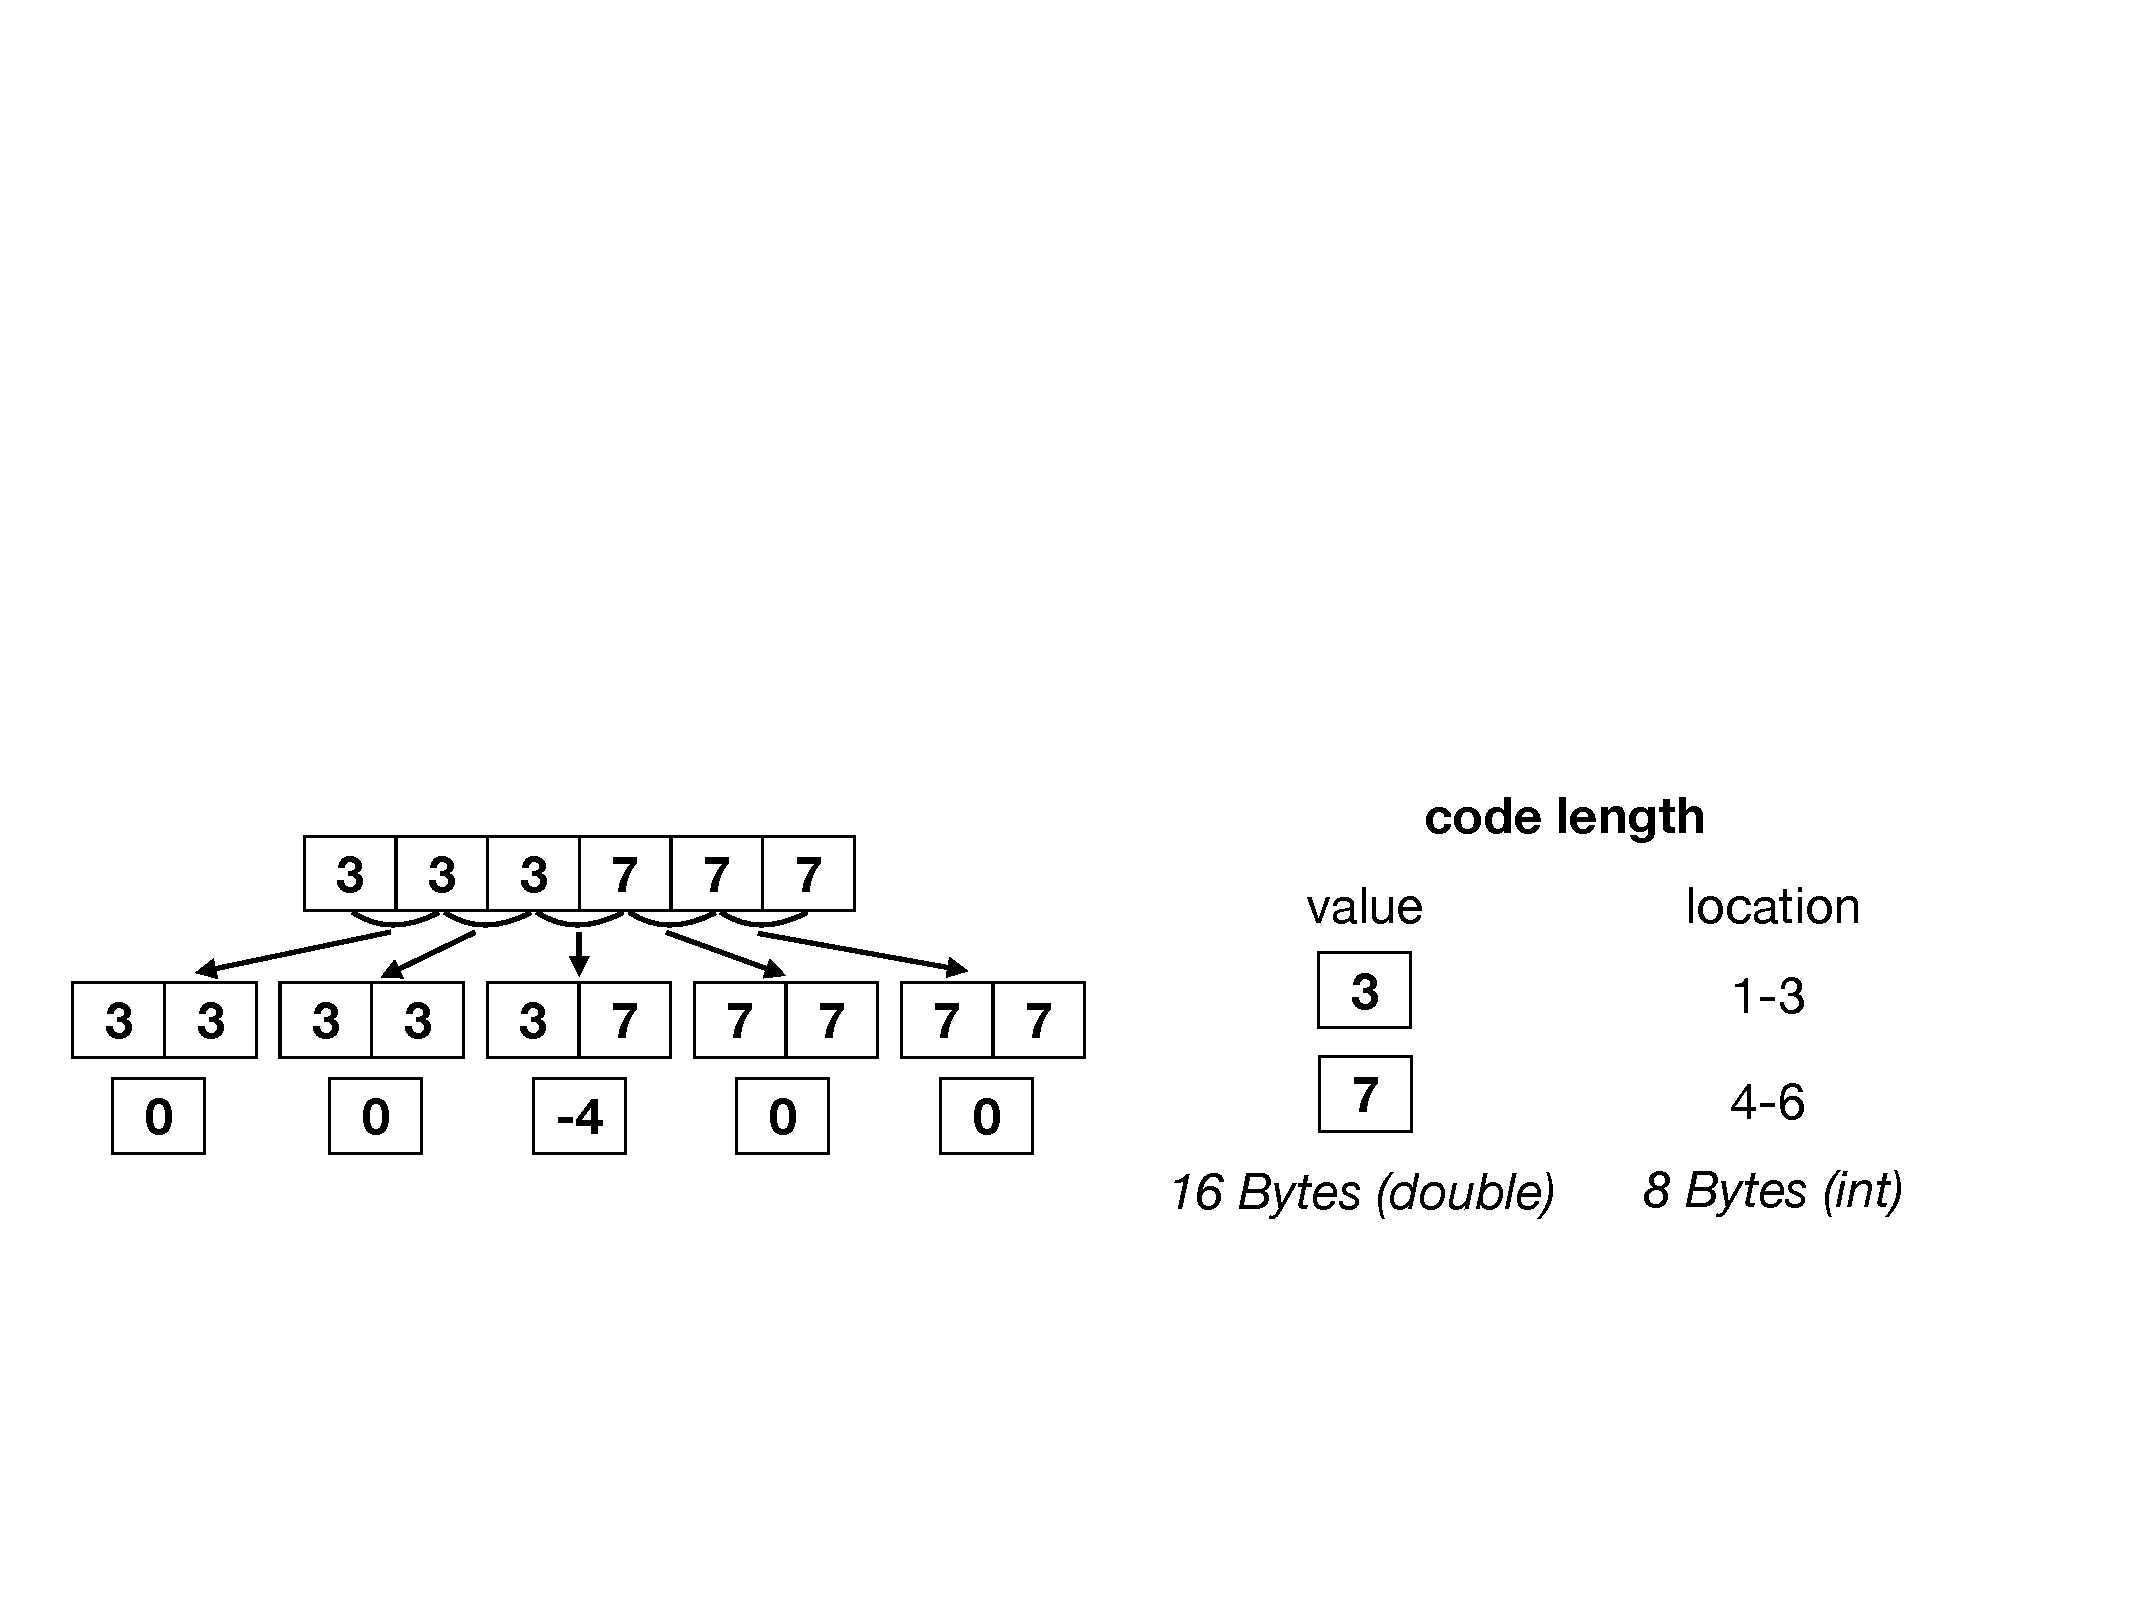
\includegraphics[width=0.98\columnwidth]{figs/figure_intro_gradient_with_clustering_details}\label{figure_intro_gradient_with_clustering_details}}
\caption{The illustrative example shows that $\nabla_{t+1}^{(n)}$ with clustering structures can be compressed by using fewer bits, and thus the code length is reduced effectively. \textbf{Our basic idea is to make the difference between  elements of $\nabla_{t+1}^{(n)}$ sparse.}}
\label{figure_intro_gradient_clustering}
\end{figure}

To improve the communication efficiency, we propose a new method to conduct the update of the parameter, which is formulated as
\begin{align}
\nonumber
\nabla_{t+1}^{(n)} = \frac{\x_t - \v}{\eta_t}, 
\end{align} where $\v$ is obtained by performing the following problem Eq. \ref{equa_update_rule_cer}.
\begin{align}
\label{equa_update_rule_cer}
\v = \argmin_{\y\in\RR^d} \lrangle {\g^{(n)}_t, \y} + \underbrace{\gamma \lrnorm{\bLambda(\y - \x_t)}_1}_{\text{communication efficient regularizer}} + \frac{\lrnorm{\y - \x_t}^2}{2\eta_t}. 
\end{align}  Here, $\g^{(n)}_t$ is a stochastic gradient, which is obtained by using the local data in the $n$-th client. The given full rank square matrix $\bLambda\in\mathbb{R}^{d\times d}$ is defined by
\begin{align}
\nonumber
\bLambda := \begin{bmatrix}
 1&  -1&  &  & \\ 
 &  1&  -1&  & \\ 
 &  &   \cdots &  & \\ 
 &  &  & 1 & -1 \\ 
 &  &  &  & 1
\end{bmatrix}.
\end{align} Notice that $\bLambda$ is a full rank square matrix, whose smallest singular value, denoted by $\sigma$,  is positive, that is, $\sigma > 0$. The proposed communication efficient regularizer is an $\ell_1$ norm square. It punishes the difference between elements of $\nabla_{t+1}^{(n)}$, and encourages them  to be small or even zero. Thus, those corresponding elements of $\nabla_{t+1}^{(n)}$ are very similar or even identical. That is, the elements of $\nabla_{t+1}^{(n)}$ own clustering structures. Exploiting the clustering structures, $\x_{t+1}$ can be compressed by using few bits, and thus improves the communication efficiency in the distributed setting.

We give a demo example to explain the communication efficient regularizer intuitively. Suppose the optimum of $\x\in\RR^4$ is $\x_{\ast} = (1, -1, 1, -1)\Tr$. If $\x_0 = (0,0,0,0)\Tr$, the communication efficient regularizer may update $\x$ as follows.
\begin{align}
\nonumber
\x_1 = & (-1,-1,1,1)\Tr, \text{ and } \bLambda(\x_1-\x_0)= (0,-2,0,1)\Tr \\ \nonumber
\x_2 = & (1,-1,1,1)\Tr, \text{ and } \bLambda(\x_2-\x_1) = (2,0,0,0)\Tr \\ \nonumber
\x_3 = & (1,-1,1,-1)\Tr, \text{ and } \bLambda(\x_3-\x_2) = (0,0,2,-2)\Tr.
\end{align} For $\x_1$, $\x_2$ and $\x_3$, there are only two different elements: `$1$' and `$-1$', which shows that there are two clusters among those elements, and their cluster centers are `$1$' and `$-1$', respectively. Meanwhile, the difference of elements between successive update, e.g., $\bLambda(\x_2-\x_1)$, contains as least two $0$s. It explains our basic idea, that is, to let the difference between elements of successive update, i.e., $\bLambda(\x^{(n)}_{t+1}-\x_t)$, be sparse. 
 
Note that there is a trade-off between the accuracy and communication efficiency. When elements of a gradient are partitioned into more clusters, the higher accuracy of the gradient is guaranteed. Meanwhile, the gradient has to be encoded by using more bytes, thus leading to the decrease of the communication efficiency.  

We take an example for more explanation. We conduct logistic regression on the \textit{covtype} dataset. $\nabla_{t+1}^{(n)}$ has $55$ elements. As illustrated in Figure \ref{figure_illustrative_communication_efficient_clustering}, the x-axis represents the elements, and the y-axis represents values of an element. When the basic gradient descent method, that is $\gamma = 0$. is used to yield $\nabla_{t+1}^{(n)}$, the top-left sub-figure shows that its elements are usually different. But, when the communication efficient regularizer is used to update $\nabla_{t+1}^{(n)}$, the top-right sub-figure shows that its elements can be partitioned into multiple clusters.  When k-means clustering is furthermore conducted on those elements, the bottom-left and bottom-right sub-figures show that those elements can be represented with $k=4$ and $k=3$ cluster centers, respectively.  

\begin{algorithm}[!t]
    \caption{Communication efficient update of personalized component on the $n$-th client for the $t+1$ iteration.}
    \label{algo_xxx}
    \begin{algorithmic}[1]
        \Require A positive $\gamma$ to improve communication efficiency.
        \State Receive the parameter $\y_t^{(n)} := \M\x_t + \N\z_t^{(n)}$ from the server.
        \State Randomly sample an instance $\a\sim\Dcal_n$, and compute the stochastic gradient $\g^{(n)}_t = \nabla f(\y_t^{(n)};\a)$ with $\a\sim\Dcal_n$.
        \State Compute $\v$ by performing:
        \begin{align}
        \nonumber
        \v = \argmin_{\y\in\RR^d} \lrangle {\g^{(n)}_t, \y} + \gamma \lrnorm{\bLambda(\y - \x_t)}_1 + \frac{\lrnorm{\y - \x_t}^2}{2\eta_t}. 
       \end{align} 
       \State Obtain the communication efficient update of local model by performing:
       $$\nabla_{t+1}^{(n)} = \frac{\x_t - \v}{\eta_t}.$$
       \State Send $\nabla_{t+1}^{(n)}$ to the server.
    \end{algorithmic}
\end{algorithm} 

\begin{align}
\nonumber
\nabla_{t+1}^{(n)} = \frac{\x_t - \v}{\eta_t}, 
\end{align} where $\v$ is obtained by performing the following problem Eq. \ref{equa_update_rule_cer}.
\begin{align}
\nonumber
\v = \argmin_{\y\in\RR^d} \lrangle {\g^{(n)}_t, \y} + \gamma \lrnorm{\bLambda(\y - \x_t)}_1 + \frac{\lrnorm{\y - \x_t}^2}{2\eta_t}. 
\end{align} 



\begin{figure}[!]
\setlength{\abovecaptionskip}{0pt}
\setlength{\belowcaptionskip}{0pt}
\centering 
\subfigure{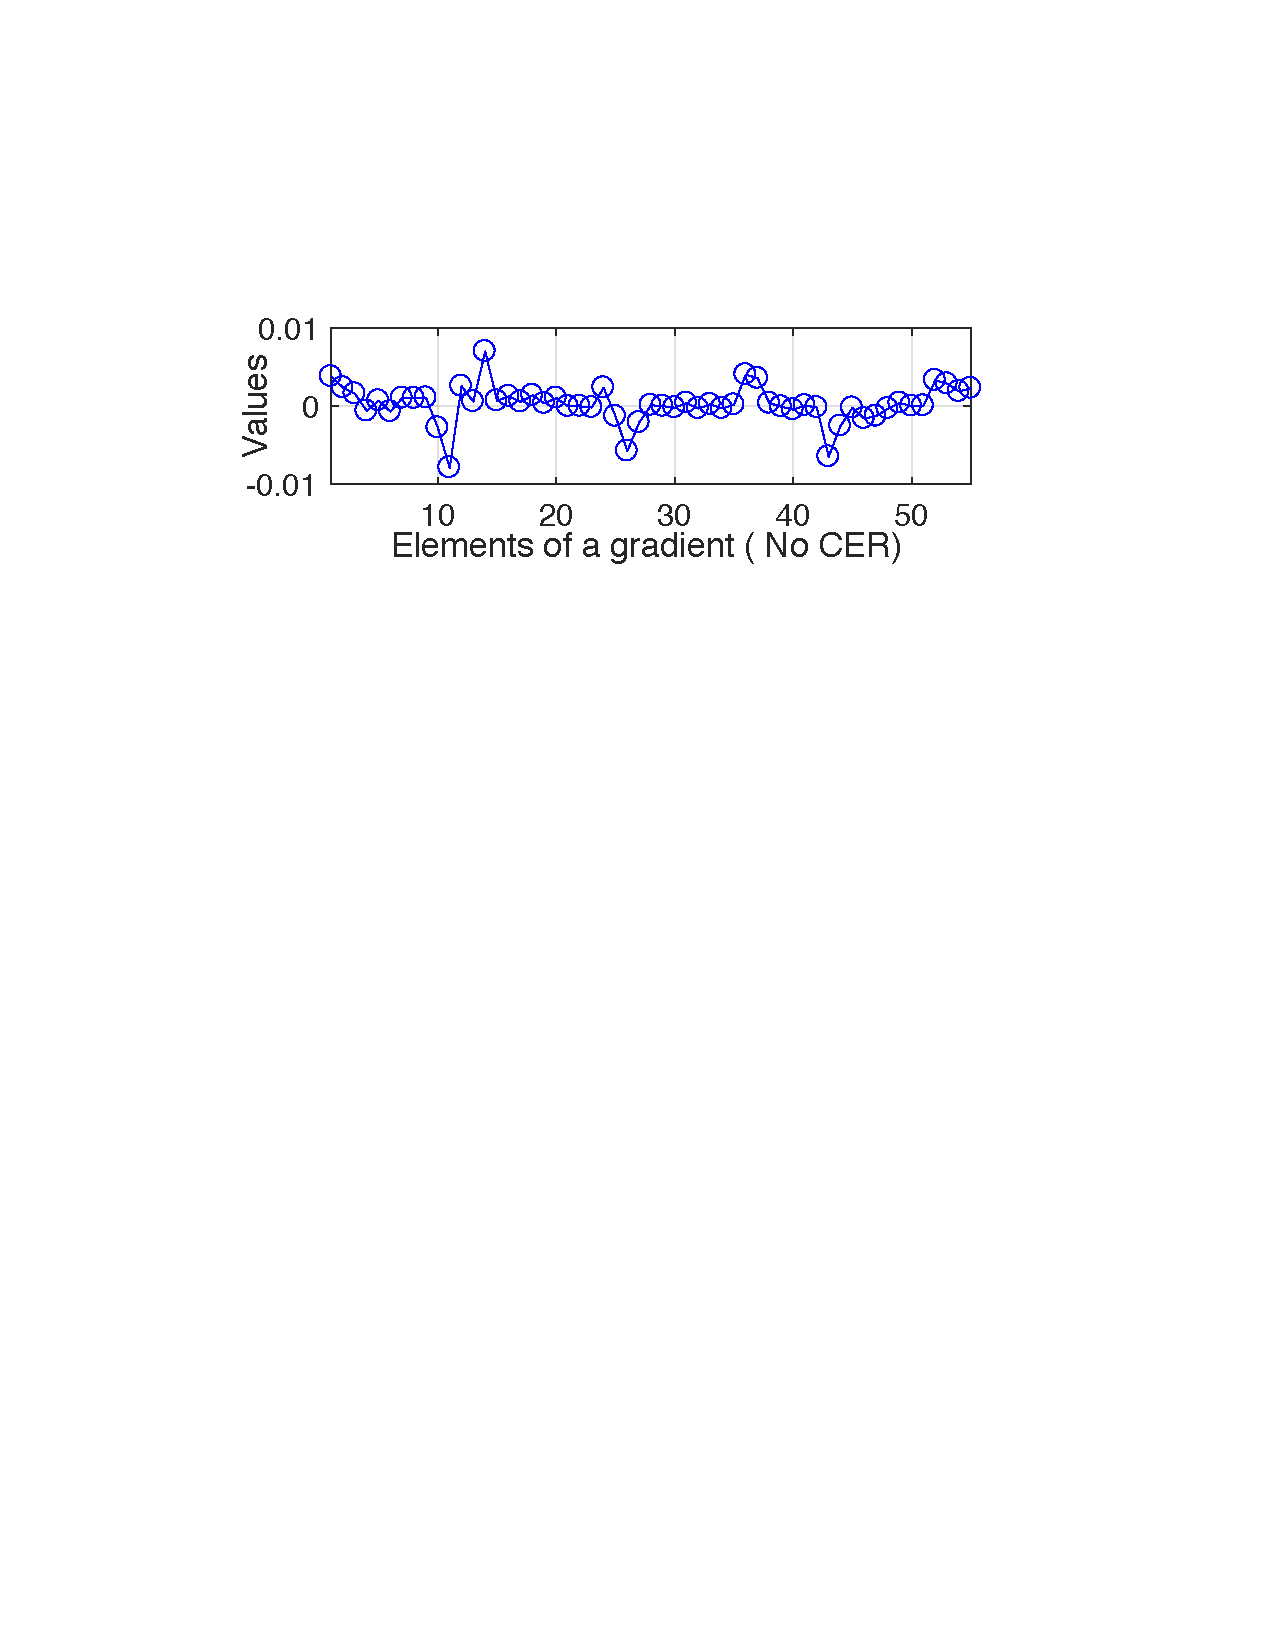
\includegraphics[width=0.47\columnwidth]{figs/figure_illustrative_communication_efficient_clustering_1}\label{figure_illustrative_communication_efficient_clustering_1}}
\subfigure{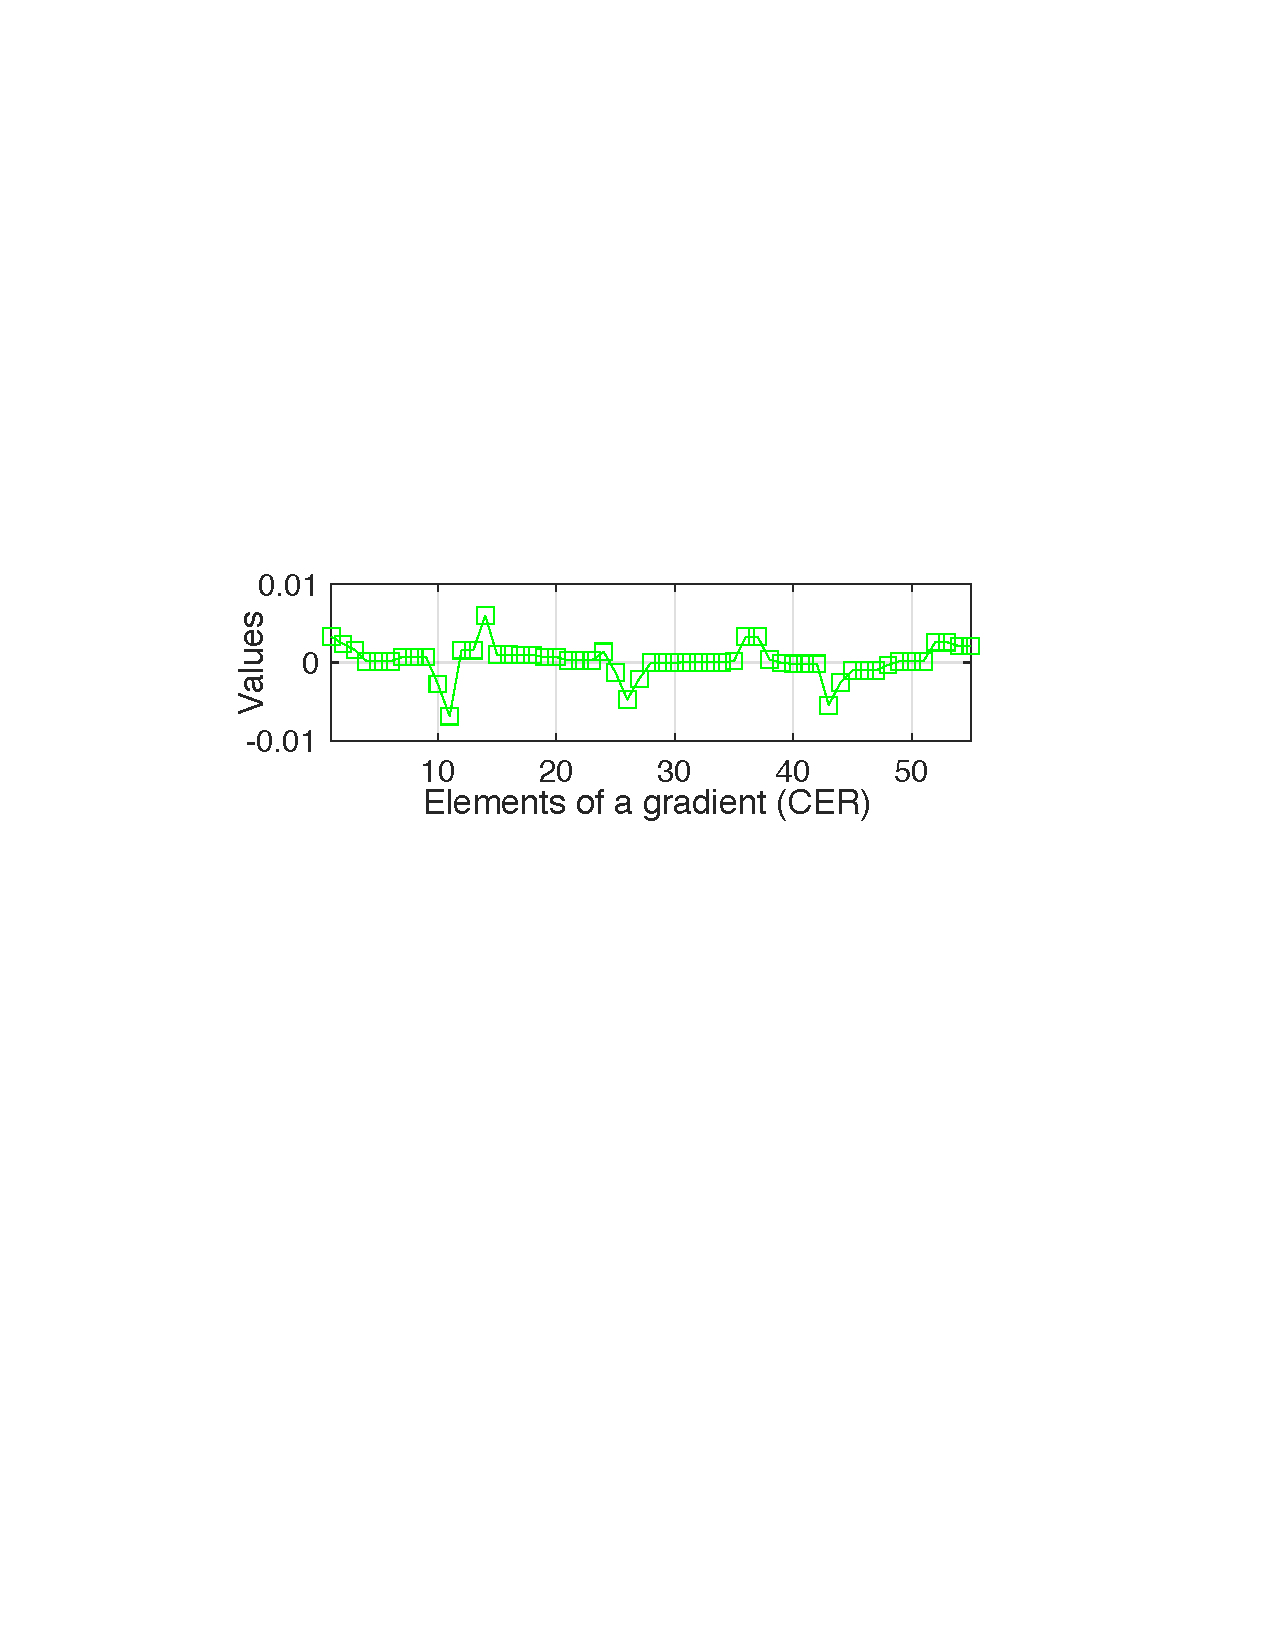
\includegraphics[width=0.47\columnwidth]{figs/figure_illustrative_communication_efficient_clustering_2}\label{figure_illustrative_communication_efficient_clustering_2}}
\subfigure{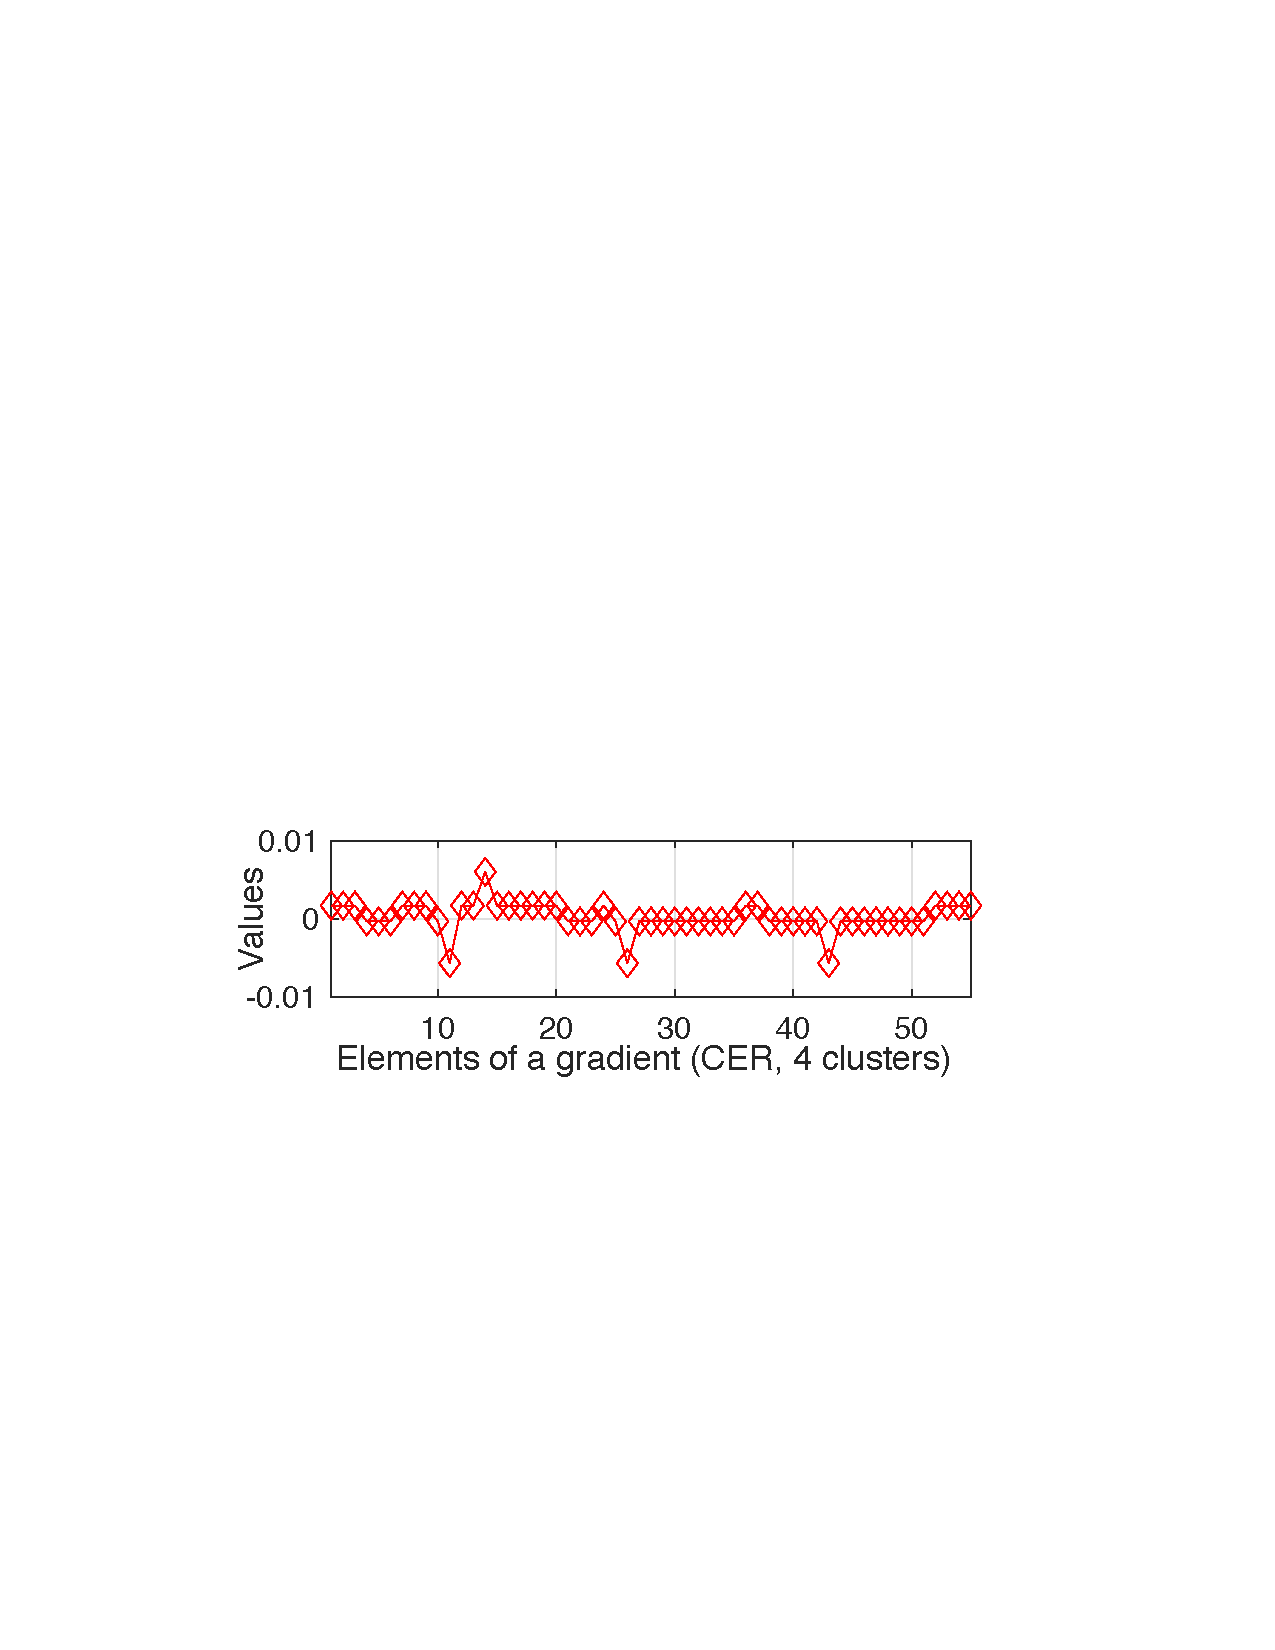
\includegraphics[width=0.47\columnwidth]{figs/figure_illustrative_communication_efficient_clustering_3}\label{figure_illustrative_communication_efficient_clustering_3}}
\subfigure{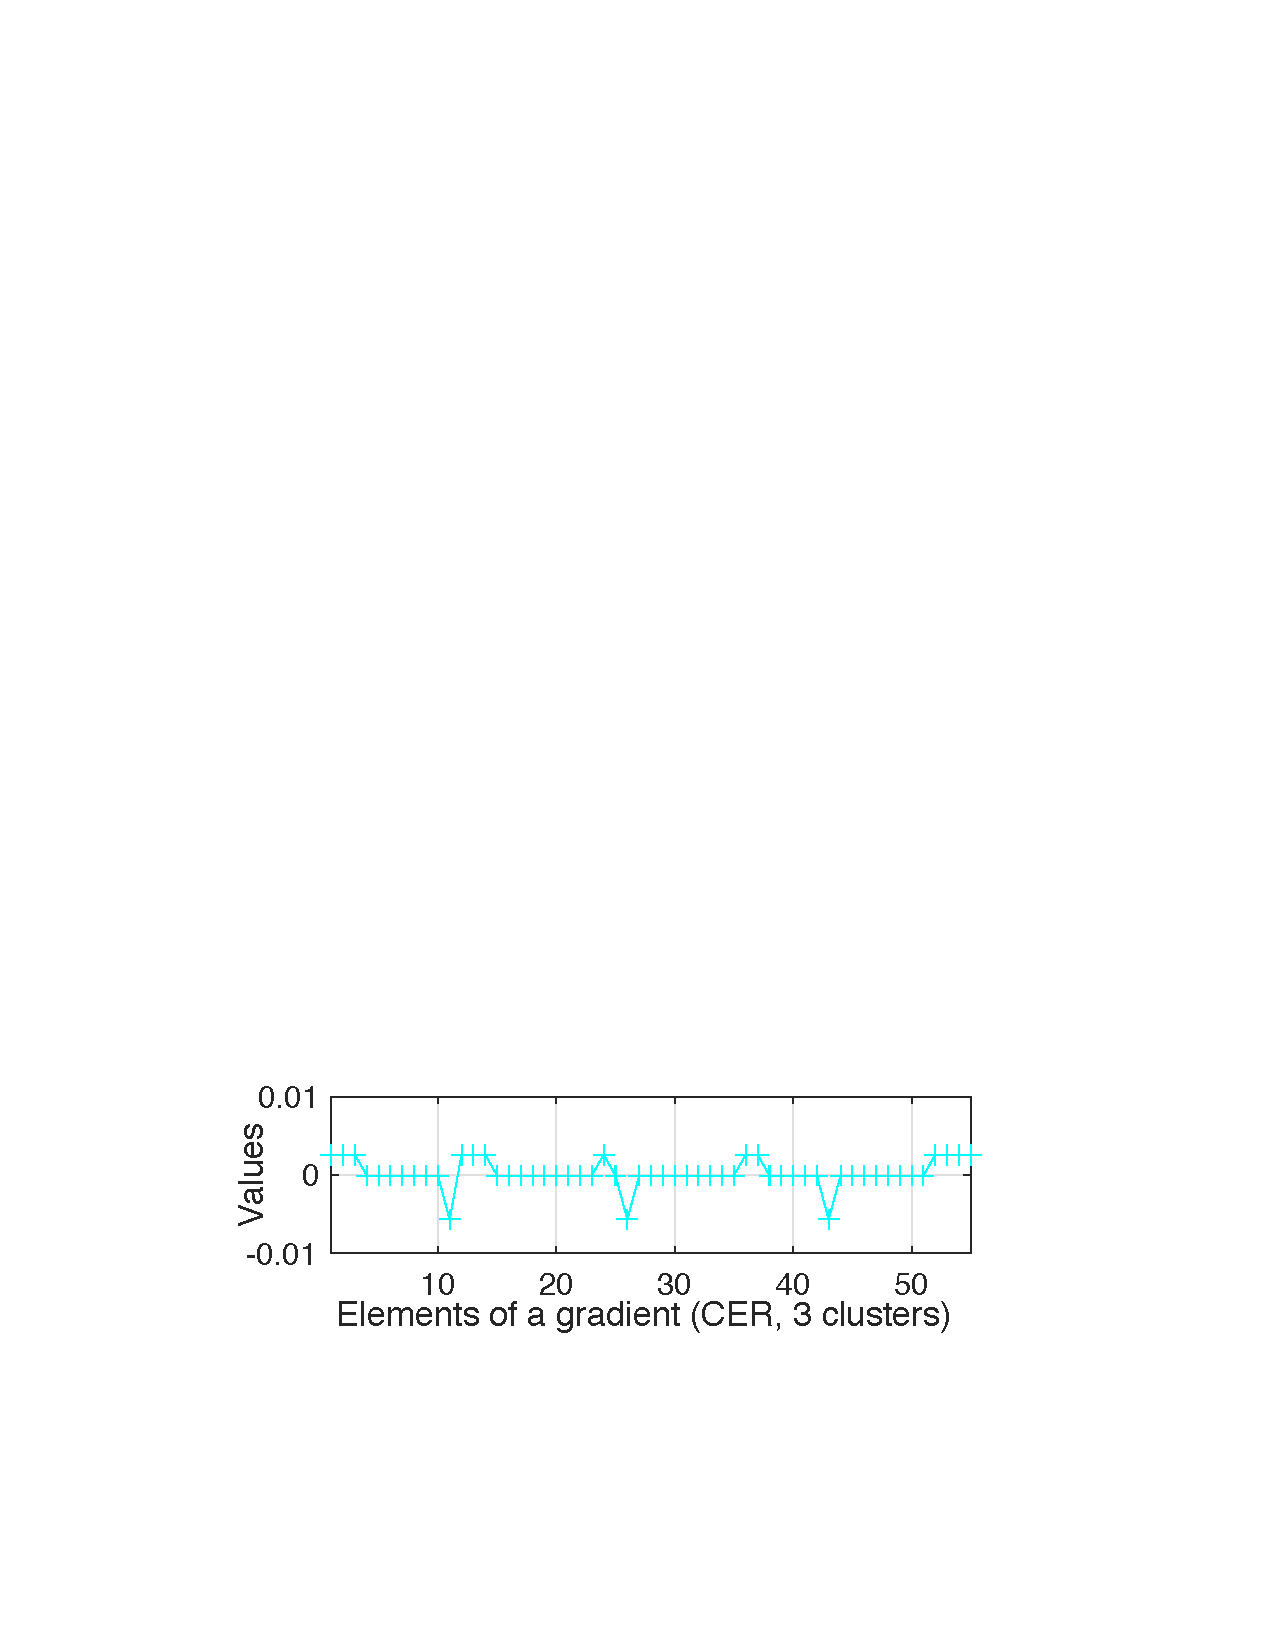
\includegraphics[width=0.47\columnwidth]{figs/figure_illustrative_communication_efficient_clustering_4}\label{figure_illustrative_communication_efficient_clustering_4}}
\caption{Comparison of elements of $\nabla_{t+1}^{(n)}$. The first sub-figure is plotted by using the classic gradient descent method without the communication efficient regularizer. The second sub-figure is plotted by using our method. The third and fourth sub-figures are plotted by using our method and the k-means clustering with $k=3$ and $k=4$, respectively.  }
\label{figure_illustrative_communication_efficient_clustering}
\end{figure}

\section{Computation Efficient Update of Model}

\subsection{Efficient update of $\x$} 

When the server collects $\nabla_{t+1}^{(n)}$ from client, the sharing component $\x$ is updated by performing as follows.
\begin{align}
\nonumber
\x_{t+1} = \argmin_{\substack{\x\in\RR^{d_1}}}  \lrangle{\frac{1}{N}\sum_{n=1}^N\M^{-1}\nabla_{t+1}^{(n)}, \x} + \frac{1}{2\eta_t}\lrnorm{\x - \x_t}^2.
\end{align} Since it is a unconstrained optimization problem, it equals to the following update rule.
\begin{align}
\nonumber
\x_{t+1} = \x_t - \eta_t \lrincir{\frac{1}{N}\sum_{n=1}^N\M^{-1}\nabla_{t+1}^{(n)}}.
\end{align} That is, the sharing component $\x$ can be updated with low computational cost.

\subsection{Efficient update of $\Z$} 

Denote 
\begin{align}
\nonumber
h(\Z) :=  \frac{\1_d^\top\lrincir{\G_t \odot \Z}\1_N}{N} + \frac{1}{2\eta_t}\lrnorm{\Z - \Z_t}_F^2.
\end{align} The update of $\Z$ can be formulated by the following problem.
\begin{align}
\nonumber
\min_{\substack{\Z\in\RR^{d_2\times N}, \W\in\RR^{d_2\times M}}} H(\Z, \W) := h(\Z) + \lambda \lrnorm{\W}_{1,p},
\end{align} subject to:
\begin{align}
\nonumber
\W = \Z\Q.
\end{align} Denote the augmented Lagrangian multiplier of $H(\Z, \W)$ by $L(\Z, \W, \bOmega)$, and we have 
\begin{align}
\nonumber
& L(\Z, \W, \bOmega) \\ \nonumber
:= & h(\Z) + \lambda \lrnorm{\W}_{1,p} + \1_{d_2}^\top(\bOmega \odot (\W - \Z\Q))\1_M + \frac{\rho}{2}\lrnorm{\W - \Z\Q}_F^2.
\end{align} 

\textbf{Update of $\Z$.} Given $\W_k$ and $\bOmega_k$, $\Z_{k+1}$ is obtained by performing the following problem.
\begin{align}
\nonumber
& \Z_{k+1}  = \argmin_{\Z\in\RR^{d_2\times N}} L(\Z, \W_k, \bOmega_k) & \\ \nonumber
= & \argmin_{\Z\in\RR^{d_2\times N}} h(\Z) - \1_{d_2}^\top(\bOmega_k \odot  (\Z\Q))\1_M + \frac{\rho}{2}\lrnorm{\W_k - \Z\Q}_F^2.
\end{align} Since it is unconstrained optimization problem, we can obtain $\Z_{k+1}$ as follows.
\begin{align}
\nonumber
\frac{\G_t}{N} + \frac{\Z_{k+1} - \Z_t}{\eta_t} -\bOmega_k\Q^\top + \rho (\Z_{k+1}\Q - \W_k)\Q^\top = \0
\end{align} That is, we have 
\begin{align}
\nonumber
& \Z_{k+1} \\ \nonumber
= & \left [ \eta_t\lrincir{\bOmega_k\Q^\top-\frac{\G_t}{N}+\rho\W_k\Q^\top}+\Z_t \right ]\lrincir{\I_N+\eta_t\rho\Q\Q^\top}^{-1}.
\end{align}

\textbf{Update of $\W$.} Given $\Z_{k+1}$ and $\bOmega_k$, $\W_{k+1}$ is obtained by performing the following problem.
\begin{align}
\nonumber
& \W_{k+1} = \argmin_{\W\in\RR^{d_2 \times M}} L(\Z_{k+1}, \W, \bOmega_k) \\ \nonumber
= & \argmin_{\W\in\RR^{d_2 \times M}} \lambda \lrnorm{\W}_{1,p} + \1_{d_2}^\top(\bOmega_k \odot \W)\1_M + \frac{\rho}{2}\lrnorm{\W - \Z_{k+1}\Q}_F^2 \\ \nonumber
= & \argmin_{\W\in\RR^{d_2 \times M}} \lambda \lrnorm{\W}_{1,p} + \frac{\rho}{2}\lrnorm{\W - \lrincir{\Z_{k+1}\Q - \frac{1}{\rho}\bOmega_k}}_F^2 \\ \nonumber
= & \Prox_{\frac{\rho}{\lambda}, \lrnorm{\cdot}_{1,p}}\lrincir{\Z_{k+1}\Q - \frac{1}{\rho}\bOmega_k}.
\end{align}  Here, $\Prox$ represents the \textit{proximal operator}, which is defined by 
\begin{align}
\nonumber
\Prox_{\nu, \phi}(\a) := \argmin_{\b} \phi(\b) + \frac{\nu}{2}\lrnorm{\b - \a}^2.
\end{align} Recall that $\lrnorm{\cdot}_{1,p}$ is the sum of norms, its proximal operator has a closed form \cite{xx}. Specifically, for the $m$-th column with $m\in\{1,2, ..., M\}$ of $\W_{k+1}$ is obtained by performing:
\begin{align}
\nonumber
& [\W_{k+1}]_{:,m} = \left [ \Prox_{\frac{\rho}{\lambda}, \lrnorm{\cdot}_{1,p}}\lrincir{\Z_{k+1}\Q - \frac{1}{\rho}\bOmega_k} \right ]_{:,m} \\ \nonumber
=& \lrincir{1\mathrm{-} \frac{1}{\lrnorm{\frac{\rho}{\lambda} \Z_{k+1}\Q_{:, m} \mathrm{-} \frac{1}{\lambda}[\bOmega_k]{:, m}}_q}}_\mathrm{+} \lrincir{\Z_{k+1}\Q_{:, m} \mathrm{-} \frac{1}{\rho}[\bOmega_k]_{:, m}},
\end{align} where $[\A]_{:,m}$ represents the $m$-th column of $\A$, and $\lrnorm{\cdot}_q$ is the dual norm of $\lrnorm{\cdot}_p$ such that $\frac{1}{p}+\frac{1}{q} = 1$.

\textbf{Update of $\bOmega$.} Given $\Z_{k+1}$ and $\W_{k+1}$, $\bOmega_{k+1}$ is obtained by performing the following problem.
\begin{align}
\nonumber
\bOmega_{k+1}  = \bOmega_k + \rho \lrincir{\W_{k+1} - \Z_{k+1}\Q}.
\end{align} 

\begin{algorithm}[!]
    \caption{Computation Efficient Update of $\Z$.}
    \label{algo_efficient_update_Z}
    \begin{algorithmic}[1]
        \Require The number of total iterations $K$, a positive $\rho$, and the initial model $\Z_t$.
           \For {$k=0,1,2, ..., K-1$}
            \State Update $\Z_{k+1}$ by performing:
            \begin{align}
            \nonumber
            & \Z_{k+1} \\ \nonumber
            = & \left [ \eta_t\lrincir{\bOmega_k\Q^\top\mathrm{-}\frac{\G_t}{N}\mathrm{+}\rho\W_k\Q^\top}\mathrm{+}\Z_t \right ]\lrincir{\I_N+\eta_t\rho\Q\Q^\top}^{-1}.
            \end{align}
            \State Update the $m$-th column of $\W_{k+1}$, that is $[\W_{k+1}]_{:,m}$ by performing:
            \begin{align}
	   \nonumber
	   & [\W_{k+1}]_{:,m} \\ \nonumber
	   \mathrm{=}& \left [1\mathrm{-} \frac{1}{\lrnorm{\frac{\rho}{\lambda} 		          \Z_{k+1}\Q_{:, m} \mathrm{-} \frac{1}{\lambda}[\bOmega_k]{:, m}}_q}\right]_\mathrm{+} \left[ \Z_{k+1}\Q_{:, m} \mathrm{-} \frac{[\bOmega_k]_{:, m}}{\rho}\right],
	\end{align} 
           \State Update $\bOmega_{k+1}$ by performing:
            $$\bOmega_{k+1}  = \bOmega_k + \rho \lrincir{\W_{k+1} - \Z_{k+1}\Q}.$$
            \State \EndFor
        \Return $\Z_K$.
      \end{algorithmic}
\end{algorithm}

\begin{algorithm}[!]
    \caption{Computation Efficient Training of personalized models on the server.}
    \label{algo_xxx}
    \begin{algorithmic}[1]
        \Require The number of total iterations $T$, and the initial parameter $\x_1$.
        %\algotext{\textbf{On the server:}}
        \State Deliver the parameter $\y_1^{(n)} = \M\x_1 + \N\z_1^{(n)}$ to all client $n$ with $n\in\{1,2, ..., N\}$.
        \For {$t=1,2, ..., T$}
            \State Collect stochastic gradient $\G_t = \left [ \g_t^{(1)}, \g_t^{(2)}, ..., \g_t^{(N)} \right ]$ from all client $n$ with $n\in\{1,2, ..., N\}$.
            \State Update the global parameter $\x$ by performing:
            $$ \x_{t+1} = \x_t - \eta_t \lrincir{\frac{1}{N}\sum_{n=1}^N\M^{-1}\nabla_{t+1}^{(n)}}. $$
           \State Update the personalized model $\Z_{t+1}$ according to Algorithm \ref{algo_efficient_update_Z}.
            \State Deliver the parameter $\y_{t+1}^{(n)} = \M\x_{t+1} + \N\z_{t+1}^{(n)}$ to every client.
        \EndFor
        \Return $\x_{T+1}^{(n)} = \M\x_{T+1} + \N\z_{T+1}^{(n)}$ with $n\in\{1,2, ..., N\}$.
      \end{algorithmic}
\end{algorithm} 






\section{Empirical Studies}









\section*{Acknowledgment}
This work was supported by the xx. 



\bibliographystyle{IEEEtran}  
\bibliography{reference}


%\begin{IEEEbiography}[{\includegraphics[width=1in,height=1.25in,clip,keepaspectratio]{Yawei.pdf}}]{Yawei Zhao} is currently a Ph.D. candidate in Computer Science from the National University of Defense Technology, China. He received his B.E. degree and M.S. degree in Computer Science from the National University of Defense Technology, China, in 2013 and 2015, respectively. His research interests include asynchronous and parallel optimization algorithms, pattern recognition and machine learning.
%[{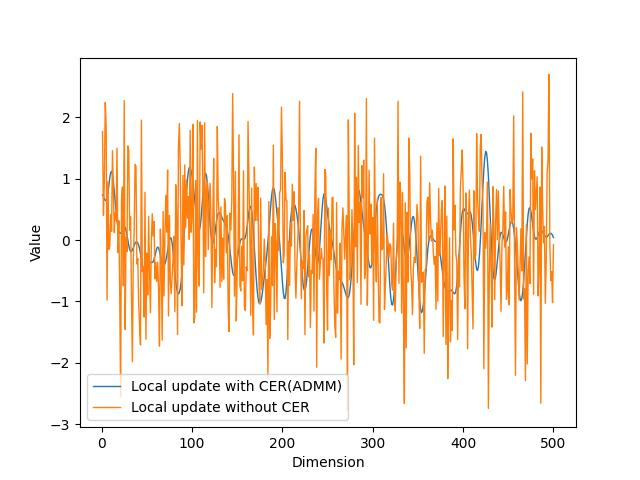
\includegraphics[width=1in,height=1.25in,clip,keepaspectratio]{xxx.pdf}}]{Yawei Zhao} is currently a Ph.D. candidate in Computer Science from the National University of Defense Technology, China. He received his B.E. degree and M.S. degree in Computer Science from the National University of Defense Technology, China, in 2013 and 2015, respectively. His research interests include asynchronous and parallel optimization algorithms, pattern recognition and machine learning.
%[{\includegraphics[width=1in,height=1.25in,clip,keepaspectratio]{jiliu.jpg}}]{Ji Liu} is currently a Ph.D. candidate in Computer Science from the National University of Defense Technology, China. He received his B.E. degree and M.S. degree in Computer Science from the National University of Defense Technology, China, in 2013 and 2015, respectively. His research interests include asynchronous and parallel optimization algorithms, pattern recognition and machine learning.
%\end{IEEEbiography}




\end{document}


